% arara: pdflatex: { options: ["--synctex=1"] }
% arara: biber if found('log', 'LaTeX Warning: There were undefined references.') || changed('references.bib')
% arara: pdflatex: { synctex: yes } until !found('log', 'undefined references')

%%%
 % File: /main.tex
 % Created Date: Monday, May 6th 2024
 % Author: Zihan
 % -----
 % Last Modified: Monday, 10th February 2025 9:37:30 pm
 % Modified By: the developer formerly known as Zihan at <wzh4464@gmail.com>
 % -----
 % HISTORY:
 % Date      		By   	Comments
 % ----------		------	---------------------------------------------------------
%%%

\documentclass[journal]{IEEEtran}
\usepackage{amsmath,amsfonts}
\usepackage{algorithmic}
\usepackage{algorithm}
\usepackage{array}
% \usepackage[caption=false,font=normalsize,labelfont=sf,textfont=sf]{subfig}
\usepackage{textcomp}
\usepackage{stfloats}
\usepackage{url}
\usepackage{verbatim}
\usepackage{graphicx}
% \usepackage{cite} % conflicts with biblatex
\usepackage{subcaption} % for subfigures
\usepackage{hyperref} % for hyperlinks
\usepackage{cleveref} % for \cref
\usepackage{doi}
% autocite
\usepackage{color}
\usepackage{csquotes}
% theorems
\usepackage{amsthm}
\usepackage{enumitem}
\newtheorem{theorem}{Theorem}
\newtheorem{lemma}{Lemma}
\newtheorem{definition}{Definition}
\newtheorem{assumption}{Assumption}
\newtheorem{corollary}{Corollary}
\newtheorem{proposition}{Proposition}

% Cref for lemma
\crefname{lemma}{lemma}{lemmas}
\Crefname{lemma}{Lemma}{Lemmas}
\crefname{assumption}{assumption}{assumptions}
\Crefname{assumption}{Assumption}{Assumptions}
\crefname{definition}{definition}{definitions}
\Crefname{definition}{Definition}{Definitions}
\crefname{corollary}{corollary}{corollaries}
\Crefname{corollary}{Corollary}{Corollaries}
\crefname{proposition}{proposition}{propositions}
\Crefname{proposition}{Proposition}{Propositions}

\hyphenation{op-tical net-works semi-conduc-tor IEEE-Xplore}

% image path: images/
\graphicspath{ {images/} }

\newcommand{\SCCcite}{\cite{dhillon2001CoclusteringDocumentsWords}}
\newcommand{\PNMTFcite}{\cite{chen2023ParallelNonNegativeMatrix}}
\newcommand{\ONMTFcite}{\cite{ding2006OrthogonalNonnegativeMatrix}}
\newcommand{\FNMTFcite}{\cite{kim2011FastNonnegativeMatrix}}

% bibliography
\usepackage[backend=biber,style=ieee]{biblatex}
\bibliography{references}
% Suppress 'url' field in 'article' entries but keep 'doi'
\renewbibmacro*{doi+eprint+url}{%
  \iftoggle{bbx:doi}
    {\printfield{doi}} % keep doi
    {}%
  \iftoggle{bbx:eprint}
    {\usebibmacro{eprint}}
    {}%
  \iftoggle{bbx:url}
    {} % suppress url
    {}%
}
% Suppress 'isbn' field
\AtEveryBibitem{%
  % exclude 'isbn' field from all entries but books
  \ifentrytype{book}{}{\clearfield{isbn}}
}

% Suppress 'issn' field
\AtEveryBibitem{%
  \clearfield{issn}
}

% add doi if available
\DeclareFieldFormat{doi}{%
  \iffieldundef{doi}{%
  }{%
    \mkbibacro{DOI}\addcolon\space
    \ifhyperref
      {\href{https://doi.org/#1}{\nolinkurl{#1}}}
      {\nolinkurl{#1}}%
  }%
}

% tables
\usepackage{booktabs}       % for professional tables
\usepackage{multirow}       % multirow in tables
\usepackage{threeparttable} % for table notes
\renewcommand{\cite}[1]{~\autocite{#1}}
\begin{document}

\title{\LARGE \bf DiMergeCo: A Scalable Framework for Large-Scale Co-Clustering with Theoretical Guarantees}

% The paper headers
% \markboth{Journal of \LaTeX\ Class Files,~Vol.~14, No.~8, August~2021}%
% {Shell \MakeLowercase{\textit{et al.}}: A Sample Article Using IEEEtran.cls for IEEE Journals}

% \IEEEpubid{0000--0000/00\$00.00~\copyright~2021 IEEE}
% Remember, if you use this you must call \IEEEpubidadjcol in the second
% column for its text to clear the IEEEpubid mark.
\author{Zihan Wu$^{1}$, Zhaoke Huang$^{2}$, and Hong Yan$^{3}$, \textit{Fellow, IEEE}% <-this % stops a space
    \thanks{This work is supported by Hong Kong Innovation and
        Technology Commission (InnoHK Project CIMDA) and Hong
        Kong Research Grants Council (Project CityU 11204821).}% <-this % stops a space
    \thanks{$^{1}$Zihan Wu (Corresponding Author) is with the Department of Electrical Engineering,
        City University of Hong Kong, Hong Kong
            {\tt\small zihan.wu@my.cityu.edu.hk}}%
    \thanks{$^{2}$Zhaoke Huang is with the Department of Electrical Engineering,
        City University of Hong Kong, Hong Kong
            {\tt\small Z.Huang@cityu.edu.hk}}%
    \thanks{$^{3}$Hong Yan, \textit{Fellow, IEEE}, is with the Department of Electrical Engineering,
        City University of Hong Kong, Hong Kong
            {\tt\small h.yan@cityu.edu.hk}}%
}
\maketitle

\begin{abstract}
    Co-clustering algorithms are effective at uncovering complex multi-dimensional data patterns by concurrently grouping rows and columns. However, existing methods face significant challenges when processing massive datasets, struggling with computational scalability and central coordinator bottlenecks. In this paper, we propose \emph{DiMergeCo}, an efficient co-clustering method for large-scale matrices. Our approach is grounded in theoretical properties of low-rank submatrices, enabling the transformation of global co-clustering into independent local problems.  First, we develop a probabilistic partitioning algorithm with theoretical guarantees to preserve co-clusters during division. Second, we design a hierarchical merging strategy to effectively aggregate local co-clustering results while eliminating the central coordinator bottleneck, achieving $O(\log n)$ communication complexity. Third, we implement our method through Message Passing Interface (MPI) with a distributed architecture where the main node only computes initial partitioning thresholds.
    Our theoretical analysis provides rigorous guarantees for co-cluster preservation and bounded convergence. Experimental evaluations on synthetic and real-world datasets demonstrate that \emph{DiMergeCo} achieves an 83\% reduction in computation time for dense matrices and scales to datasets with 685K samples, outperforming existing methods in both speed and accuracy.
\end{abstract}

\begin{IEEEkeywords}
    Co-clustering, distributed computing, matrix partitioning, hierarchical merging, large-scale data analysis.
\end{IEEEkeywords}


\section{Introduction}
\IEEEPARstart{R}{ecent} advancements in machine learning have significantly benefited from the use of large-scale datasets. Clustering, a fundamental unsupervised learning technique, plays a crucial role in the preprocessing of large-scale training data. By grouping similar data together, clustering enables refined feature recognition and intricate pattern analysis. Consequently, clustering reduces noise during model training and improves data organization, significantly boosting both the efficiency and effectiveness of large-scale models~\cite{raskutti2002CombiningClusteringCotraining, li2014ClusteringguidedSparseStructural, ghimatgar2018ImprovedFeatureSelection}. However, traditional clustering methods~\cite{lloyd1982LeastSquaresQuantization, arthur2007KmeansAdvantagesCareful, mclachlan1987MixtureModelsInference} treat all features uniformly and solely cluster either rows (samples) or columns (features), as shown in \Cref{fig:cluster}. This one-dimensional perspective fails to capture the intricate interrelationships often present in complex, high-dimensional data structures.

\textit{Co-clustering}~\cite{kluger2003SpectralBiclusteringMicroarray, yan2017CoclusteringMultidimensionalBig,wu2024AccurateDetectionEllipses} address these limitations by simultaneously grouping rows (samples) and columns (features), as shown in \Cref{fig:cocluster}. This bidirectional approach enables the discovery of hidden patterns and interdependencies between different data dimensionsCo-clustering has proven particularly valuable in domains where the interactions between different data dimensions carry crucial information. For example, in bioinformatics, co-clustering enables the simultaneous analysis of genes and experimental conditions, leading to discoveries of complex biological patterns~\cite{higham2007SpectralClusteringIts, kluger2003SpectralBiclusteringMicroarray, madeira2004BiclusteringAlgorithmsBiological, zhao2012BiclusteringAnalysisPattern, golchev2015BiclusteringAnalysisGene}.
In multimodal learning, co-clustering facilitates the integration of diverse data types, revealing intricate cross-modal patterns that enhance predictive performance~\cite{mu2022LearningHybridBehavior}.

\begin{figure}[t]
    \centering
    \begin{subfigure}[b]{0.22\textwidth}
        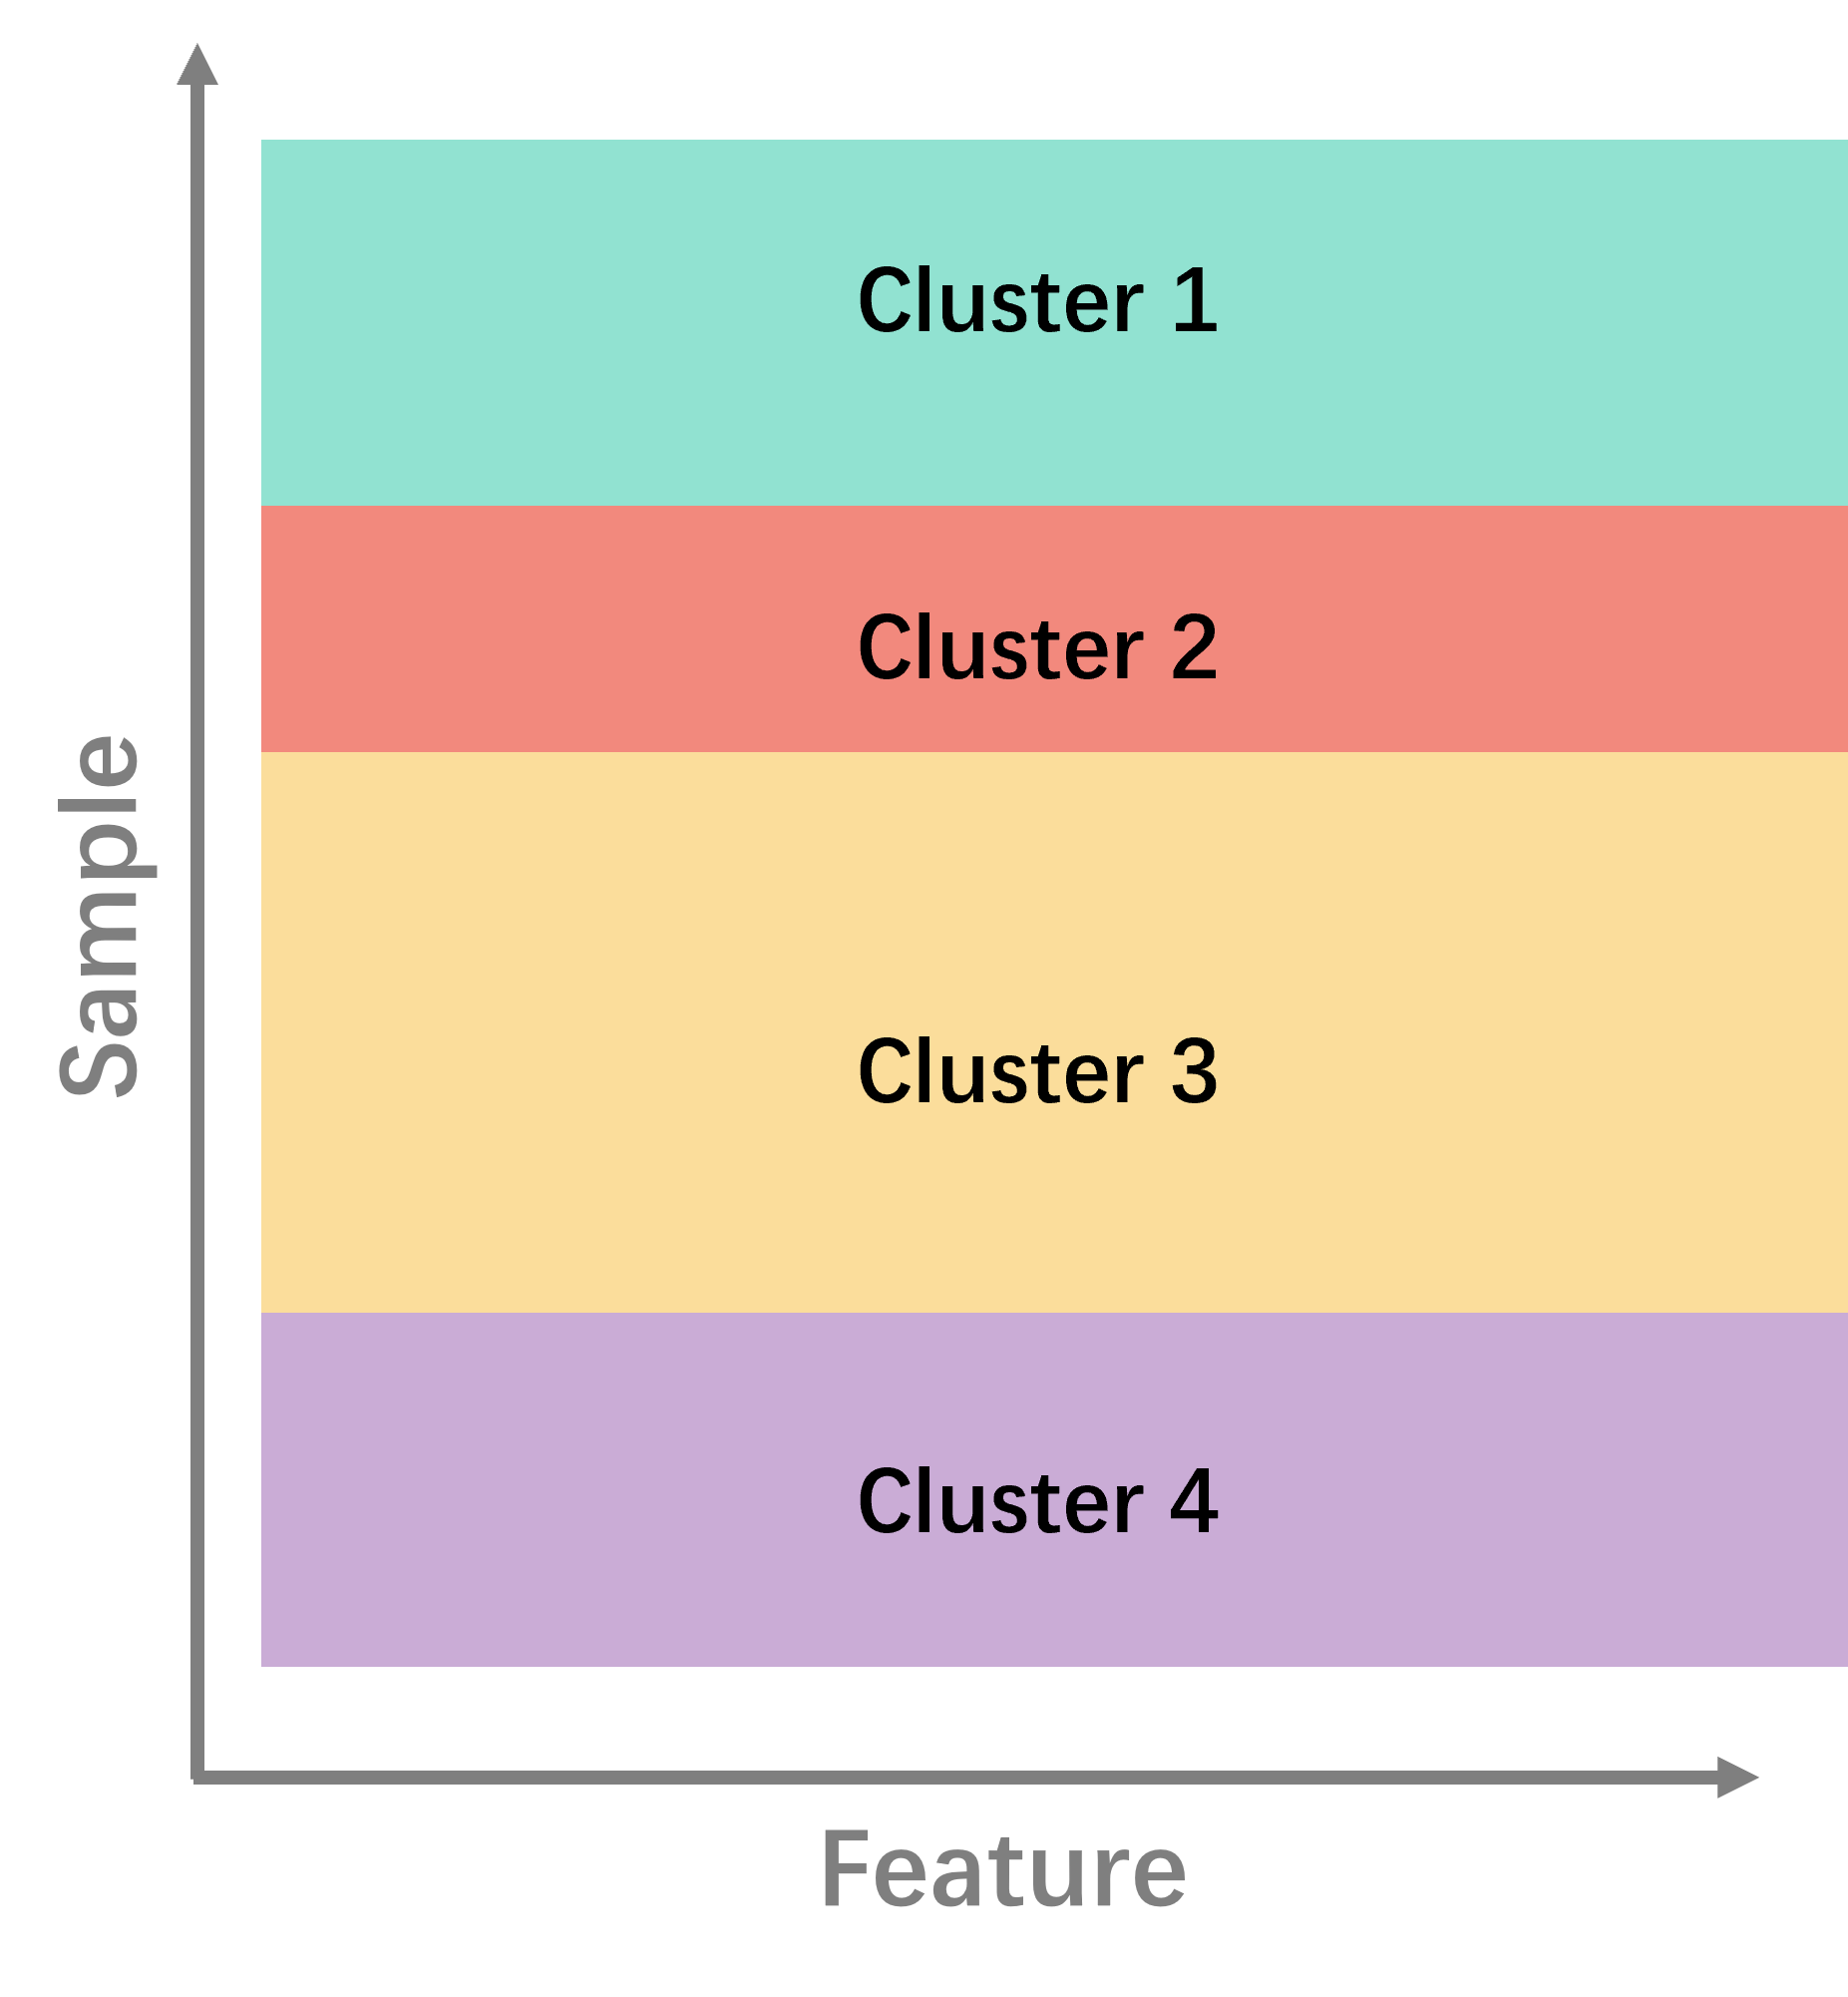
\includegraphics[width=\linewidth]{cluster.png}
        \caption{Clustering}
        \label{fig:cluster}
    \end{subfigure}
    \hfill
    \begin{subfigure}[b]{0.22\textwidth}
        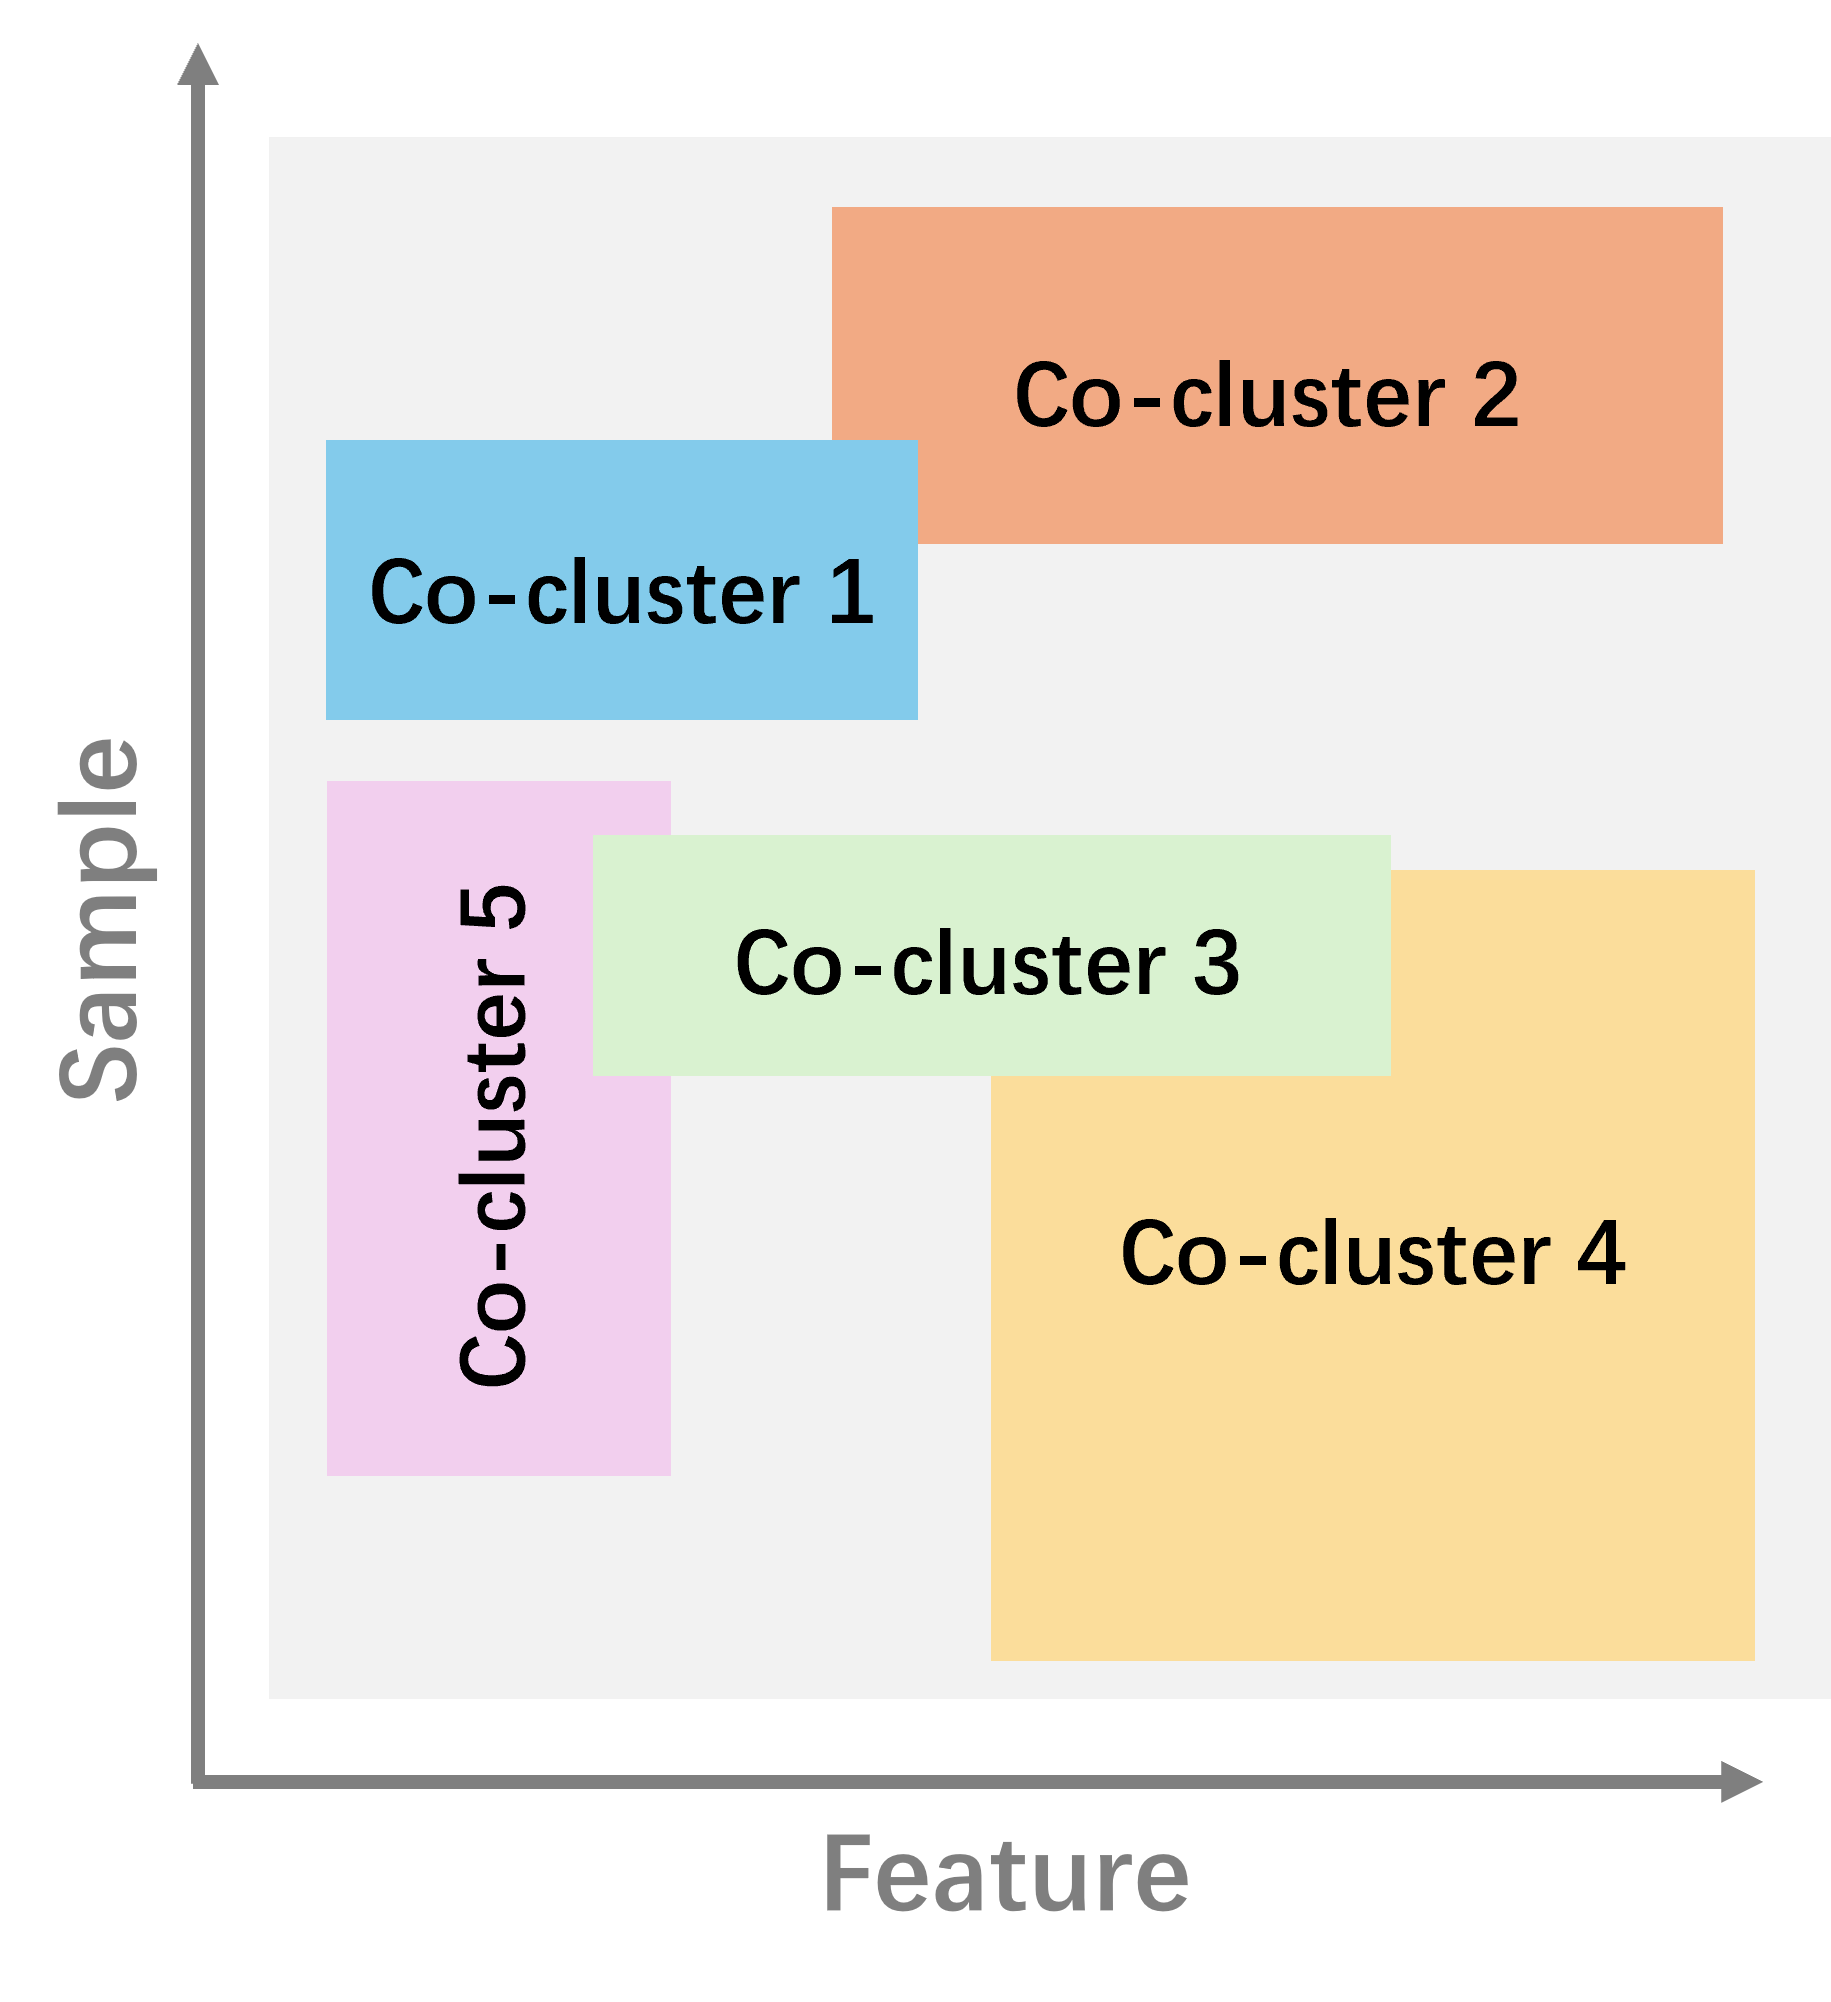
\includegraphics[width=\linewidth]{coc.png}
        \caption{Co-clustering}
        \label{fig:cocluster}
    \end{subfigure}
    \caption{An illustration of the differences between (a) Clustering and (b) Co-clustering~\cite{yan2017CoclusteringMultidimensionalBig}.}
    \label{fig:cocomparison}
\end{figure}

While co-clustering has great potential, existing co-clustering algorithms face significant challenges when applied to large-scale datasets~\cite{cheng2015CoClusterDDistributedFramework}. This challenge arises from the need to simultaneously optimize both row and column clusters, turning the problem into a multi-objective optimization task. This task involves minimizing multiple loss functions concurrently, often leading to conflicting gradients and optimization paths. These conflicts complicate the convergence process, making it difficult to achieve efficient and effective clustering~\cite{coello2007EvolutionaryAlgorithmsSolving}. Recent research has attempted to address these challenges through distributed computing approaches. Parallel Non-negative Matrix Tri-Factorization (PNMTF)~\cite{chen2023ParallelNonNegativeMatrix} employs parallelization but requires broadcasting large matrices across nodes and lacks guaranteed iteration bounds. Similarly, Co-ClusterD~\cite{cheng2015CoClusterDDistributedFramework} introduces a distributed framework but relies on its main thread to process complex co-cluster statistics, creating a central bottleneck that constrains overall system performance.

In this paper, we propose DiMergeCo, an efficient co-clustering method for analyzing large-scale matrices. Our approach is grounded in two fundamental theoretical properties. First, co-clusters manifest as low-rank submatrices in the data, representing highly correlated row-column groups~\cite{zhao2016IdentifyingMultidimensionalCoclusters}. Second, matrix algebra proves that any submatrix's rank is bounded by its parent matrix's rank~\cite{horn1985MatrixAnalysis}, ensuring the preservation of low-rank structures in submatrices. These properties reveal that preserving local co-cluster structures during partitioning enables their discovery through independent analysis of smaller submatrices. Therefore, the key challenge becomes developing an effective matrix partitioning strategy that preserves significant co-clusters during the division process.

To address this challenge, we introduce three key innovations. First, we develop a probabilistic partitioning algorithm with theoretical guarantees to preserve co-clusters during division, successfully transforming the global co-clustering problem into independent local problems while maintaining all significant patterns. Second, to effectively combine these local solutions, we design a binary tree-based hierarchical merging strategy that eliminates the central coordinator bottleneck by enabling nodes to communicate only with immediate neighbors, reducing per-node communication complexity from $O(n)$ to $O(\log n)$. Third, we develop an efficient distributed implementation through Message Passing Interface (MPI). This implementation processes million-dimensional matrices efficiently, with the main node only responsible for computing initial partitioning thresholds through a logarithmic-time algorithm.

In summary, the main contributions of this paper are:
\begin{enumerate}
    \item \textbf{Theoretically-Guaranteed Probabilistic Partitioning:} We propose a novel matrix partitioning algorithm with provable guarantees for co-cluster preservation. Our method successfully decomposes large-scale co-clustering into independent subproblems while ensuring significant patterns remain intact with high probability, supported by mathematical analysis.

    \item \textbf{Communication-Efficient Hierarchical Merging:} We develop a binary tree-based merging strategy that eliminates the central coordinator bottleneck of existing methods. This approach reduces per-node communication complexity from $O(n)$ to $O(\log n)$ while maintaining clustering quality, enabling efficient processing of large-scale datasets.

    \item \textbf{Scalable Implementation and Empirical Validation:} We implement DiMergeCo through MPI with a distributed architecture that processes million-dimensional matrices efficiently. Extensive experiments on real-world datasets demonstrate that our method significantly outperforms state-of-the-art approaches in both scalability and clustering quality.
\end{enumerate}

The remainder of this paper is organized as follows. Section \Cref{sec:related_work} discusses related work in the field of co-clustering and parallel computing. Section \Cref{sec:problem_formulation} presents the mathematical formulation and problem statement of co-clustering. Section \Cref{sec:proposed_model} details our proposed scalable co-clustering method.
Section \Cref{sec:experiment} presents the experimental evaluation of our method. Section \Cref{sec:conclusion} concludes the paper and outlines future research directions. The theoretical analysis, including error bounds, complexity analysis, and optimality conditions, is provided in \Cref{sec:appendix_theoretical_analysis}.

\section{Preliminaries and Problem Statement}
\label{sec:problem_formulation}
\subsection{Preliminaries}
Co-clustering, also known as biclustering, discovers coherent substructures by simultaneously grouping rows and columns in data matrices. This technique has broad applications in recommendation systems, gene expression analysis, and document clustering, where identifying underlying local patterns is crucial for understanding complex relationships in the data.

Given a data matrix $\mathbf{A} \in \mathbb{R}^{m \times n}$ where $m$ and $n$ denote the number of samples and features respectively, each element $a_{ij}$ represents the interaction between the $i$-th sample and $j$-th feature. We denote the sets of row and column indices as $I = \{1,2,\ldots,m\}$ and $J = \{1,2,\ldots,n\}$ respectively. The set of discovered co-clusters is represented as $\mathcal{C} = \{\mathbf{C}_k\}_{k=1}^K$, where each $\mathbf{C}_k \subseteq I \times J$ represents a submatrix exhibiting coherent patterns. For any matrix $\mathbf{A}$, its Frobenius norm is defined as $\|\mathbf{A}\|_F = \sqrt{\sum_{i=1}^m \sum_{j=1}^n a_{ij}^2}$.

Our approach is grounded in two fundamental theorems from matrix analysis that establish the theoretical basis for discovering co-clusters through matrix partitioning. The first theorem, Low-Rank Approximation, establishes that co-clusters, as coherent substructures, can be effectively approximated by low-rank matrices:

\begin{theorem}[Low-Rank Approximation~\cite{eckart1936ApproximationOneMatrix}]
    For any matrix $\mathbf{A} \in \mathbb{R}^{m \times n}$, its best rank-r approximation in Frobenius norm is given by truncating its singular value decomposition to the top r singular values:
    \begin{equation}
        \min_{\text{rank}(\hat{\mathbf{A}})=r} \|\mathbf{A} - \hat{\mathbf{A}}\|_F = \|\mathbf{A} - \sum_{i=1}^r \sigma_i \mathbf{u}_i\mathbf{v}_i^T\|_F
    \end{equation}
    where $\sigma_i$, $\mathbf{u}_i$, and $\mathbf{v}_i$ are the i-th singular value and vectors of $\mathbf{A}$.
\end{theorem}

The second theorem, Rank Monotonicity, guarantees that low-rank structures (co-clusters) are preserved in submatrices, providing the theoretical foundation for our divide-and-conquer approach:

\begin{theorem}[Rank Monotonicity\cite{horn1985MatrixAnalysis}] \label{thm:rank_monotonicity}
    For any matrix $\mathbf{A}$ and its submatrix $\mathbf{A}'$, we have:
    \begin{equation}
        \text{rank}(\mathbf{A}') \leq \text{rank}(\mathbf{A})
    \end{equation}
\end{theorem}

This property provides a theoretical guarantee that when we partition a matrix containing low-rank structures, these patterns remain discoverable within the resulting submatrices. Building on this foundation, co-clustering aims to identify groups of rows and columns that form relatively low-rank submatrices in a data matrix. Such submatrices, which we refer to as co-clusters, often represent the core relationships or patterns within high-dimensional datasets. In practice, however, large and intricate data can obscure these low-rank structures, making them challenging to detect through a single global procedure. Dividing the dataset into smaller submatrices can be highly beneficial for revealing localized low-rank patterns, since each submatrix—being smaller—tends to have an even lower rank (or be easier to approximate by low-rank factors). Many existing techniques, such as singular value decomposition or non-negative matrix factorizations, work more efficiently and accurately on these smaller blocks.

To quantify the coherence of potential co-clusters and guide the discovery process, we introduce the Singular Value Ratio Score:

\begin{definition}[Singular Value Ratio Score]
    For a matrix $\mathbf{A} \in \mathbb{R}^{M \times N}$, the score measures the dominance of the primary singular value:
    \begin{equation}
        s(\mathbf{A}) = \frac{s_1}{s_2}
    \end{equation}
    where $s_1$, $s_2$ are the largest and second largest singular values. The normalized score accounts for matrix size:
    \begin{equation}
        S(\mathbf{A}) = \frac{s(\mathbf{A})}{\|\mathbf{A}\|_F}
    \end{equation}
    A higher score indicates stronger co-cluster coherence.
\end{definition}

\subsection{Problem Statement}
\label{subsec:problem_statement}
Modern applications increasingly involve massive datasets where both dimensions exceed millions ($m, n \gg 10^6$). At this scale, traditional co-clustering methods become computationally infeasible due to the significant complexity of managing and processing such data. In particular, computing and storing the similarity matrix requires $O(mn)$ memory, and performing the corresponding eigendecomposition demands $O(mn\min(m,n))$ computational operations. The fundamental challenge, therefore, is to develop a scalable co-clustering framework that maintains high solution quality under practical computational constraints.

Formally, the co-clustering objective is defined as
\begin{equation}
    J = \sum_{k=1}^{K} \sum_{l=1}^{L} \sum_{i \in R_k} \sum_{j \in C_l} \| x_{ij} - u_{kl} \|^2,
\end{equation}
which, together with probabilistic guarantees (i.e., \(P(\text{preserve significant co-clusters}) \geq 1 - \alpha\)), ensures that the framework reliably captures the intrinsic structure of the data.

\section{The Scalable Co-clustering Method}
\label{sec:proposed_model}

\subsection{Overview}
\label{subsec:overview}
We propose DiMergeCo to address the fundamental challenges of analyzing large-scale datasets. Our approach is grounded in the observation that co-clusters represent low-rank substructures within the data matrix, capturing core relationships or patterns within high-dimensional datasets. While splitting a large matrix into smaller blocks might potentially fragment co-clusters, our framework effectively addresses this challenge through a carefully designed probabilistic partitioning strategy with theoretical guarantees for preserving co-cluster structures across multiple scales.

\Cref{fig:DiMergeCo_pipeline} shows the conceptual pipeline of our framework. The method consists of three key components, each designed to address specific challenges while maintaining theoretical guarantees.

First, we introduce a probabilistic matrix partitioning algorithm that divides large matrices into smaller, manageable submatrices. This algorithm is meticulously designed to ensure co-cluster integrity during division, addressing the risk of missing small or intricate co-clusters by estimating the likelihood of their identification. The model guarantees comprehensive data coverage and robust clustering results through theoretical bounds on detection probability.

Second, each submatrix undergoes independent co-clustering analysis. Our framework is modular, allowing the integration of any advanced co-clustering technique that can reliably identify co-clusters above a certain size. This flexibility ensures that the method can be tailored to the unique characteristics of each submatrix, optimizing clustering results while maintaining theoretical guarantees of comprehensive and accurate clustering outcomes.

Finally, we develop a novel hierarchical merging strategy that combines the co-clustering results from all submatrices into a coherent global solution. Unlike existing methods such as Non-negative Matrix Tri-Factorization (NMTF) or alternating row and column optimization approaches~\cite{wang2011FastNonnegativeMatrix}, our merging process has a bounded iteration count determined by the data size. This bounding leads to a predictable time frame for achieving the ideal result, ensuring both computational efficiency and solution quality.

The complete procedure is detailed in \Cref{alg:method}. In the following sections, we detail these three core components: the large matrix partitioning algorithm (\Cref{subsec:large_matrix_partitioning}), the local co-clustering method (\Cref{subsec:local_co_clustering}), and the hierarchical merging strategy (\Cref{subsec:hierarchical_merging}). The theoretical foundations supporting these components are then presented in \Cref{sec:theoretical_foundations}, including convergence analysis and error bounds. Finally, we demonstrate the practical effectiveness of our approach through an MPI implementation for distributed computing environments in \Cref{subsec:mpi_implementation}.

\begin{figure*}[t]
    \centering
    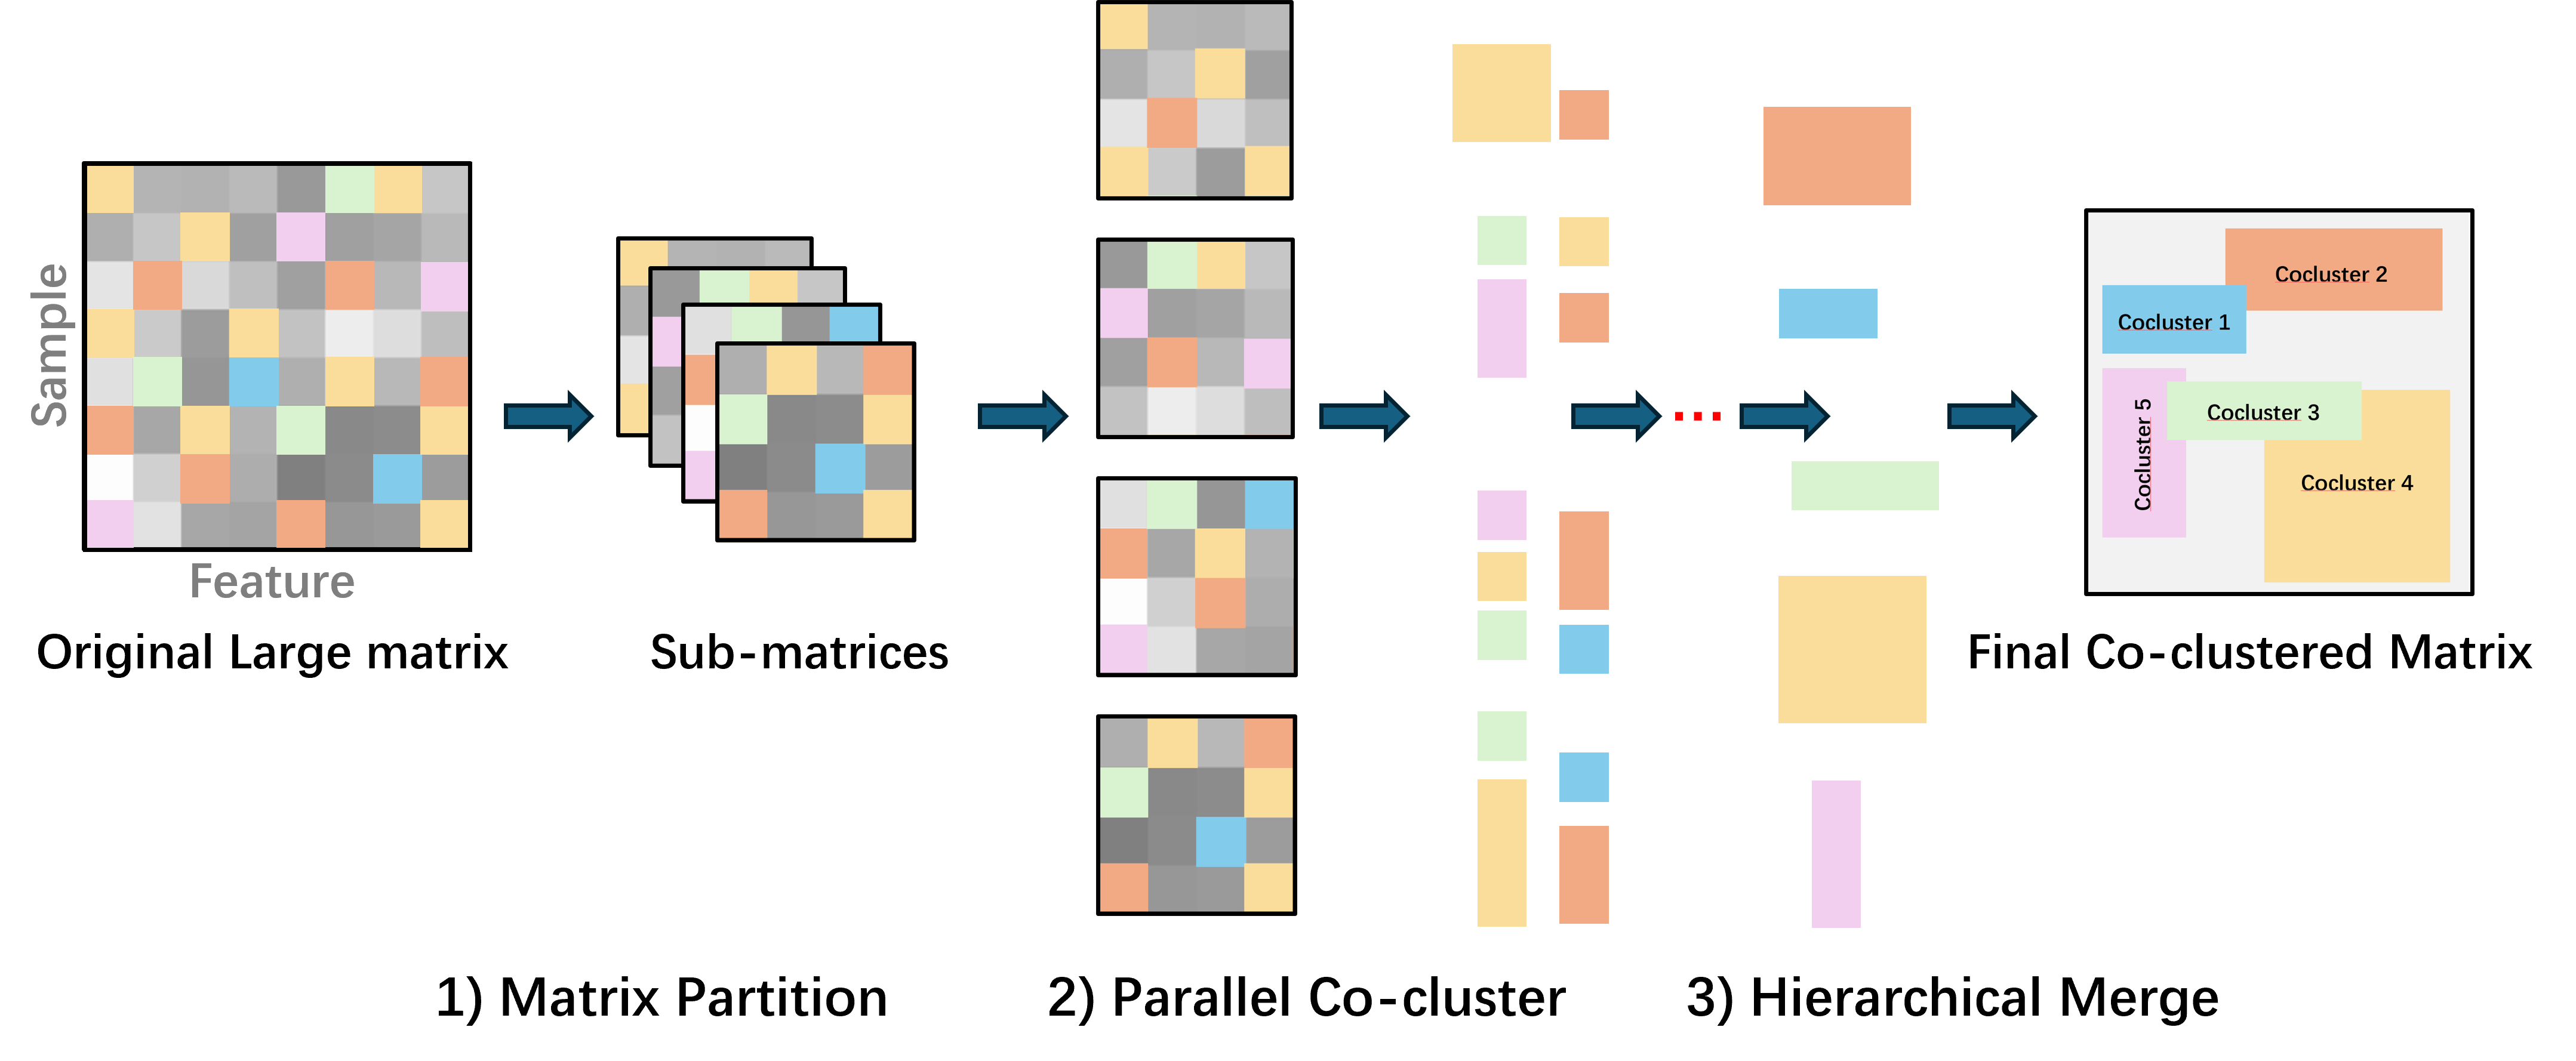
\includegraphics[width=0.8\linewidth]{workflow.png} % replace with your figure file
    \caption{High-level pipeline of the DiMergeCo framework. The data matrix is first partitioned into smaller blocks, each block is locally co-clustered in parallel, and the partial results are merged hierarchically to form the final co-clusters.}
    \label{fig:DiMergeCo_pipeline}
\end{figure*}


\begin{algorithm}[!t]
    \caption{Optimal Matrix Partition and Hierarchical Co-cluster Merging Method}\label{alg:method}
    \begin{algorithmic}[1]
        \REQUIRE{Data matrix $\mathbf{A} \in \mathbb{R}^{M \times N}$, Co-cluster set $C = \{C_k\}_{k=1}^K$, Block sizes $\{\phi_i\}_{i=1}^m$, $\{\psi_j\}_{j=1}^n$, Thresholds $T_m$, $T_n$, Sampling times $T_p$, Probability threshold $P_\text{thresh}$;}
        \ENSURE{Co-clustered result $\mathcal{C}$;}
        \STATE Initialize block set $B = \{B_{(i,j)}\}_{i=1}^m,_{j=1}^n$ based on $\phi_i$ and $\psi_j$
        \STATE Calculate $s^{(k)}$ and $t^{(k)}$ for each co-cluster $C_k$
        \FOR{$k=1$ to $K$}
        \STATE Calculate $P(\omega_k)$ for co-cluster $C_k$
        \IF{$P(\omega_k) < P_\text{thresh}$}
        \STATE Partition matrix $A$ into blocks $B$ and perform co-clustering
        \STATE Aggregate co-clustered results from each block
        \ENDIF
        \ENDFOR
        \RETURN Aggregated co-clustered result $\mathcal{C}$
    \end{algorithmic}
\end{algorithm}


\subsection{Large Matrix Partitioning}
\label{subsec:large_matrix_partitioning}
The primary challenge in co-clustering large matrices is the risk of losing meaningful co-cluster relationships when the matrix is partitioned into smaller submatrices. To address this, we introduce an optimal partitioning algorithm underpinned by a probabilistic model. This model is meticulously designed to navigate the complexities of partitioning, ensuring that the integrity of co-clusters is maintained even as the matrix is divided. The objective of this algorithm is twofold: to determine the optimal partitioning strategy that minimizes the risk of fragmenting significant co-clusters and to define the appropriate number of repartitioning iterations needed to achieve a desired success rate of co-cluster identification.

Our solution comprises three key components: a fundamental partitioning strategy based on probabilistic modeling, theoretical foundations ensuring detection guarantees, and a practical implementation framework. We present these components in the following subsections.

\subsubsection{Partitioning Strategy based on the Probabilistic Model}

Our probabilistic model serves as the cornerstone of the partitioning algorithm. It assures all co-clusters above a demarcated size threshold are identified with a high probability, guiding the partitioning process to minimize the risk of losing critical co-cluster relationships. The model is based on the following assumptions:

In the scenario where the matrix $A$ is partitioned into $m \times n$ blocks, each block has size $\phi_i \times \psi_j$, that is, $M=\sum_{i=1}^m \phi_i$ and $N=\sum_{j=1}^n \psi_j$, the joint probability of $M_{(i,j)}^{(k)}$ and $N_{(i,j)}^{(k)}$ is given by \Cref{thm:joint_probability}:
\begin{equation}
    \begin{split}
        P(M_{(i,j)}^{(k)} & < T_m, N_{(i,j)}^{(k)} < T_n)                                                                           \\
                          & = \sum_{\alpha=1}^{T_m-1} \sum_{\beta=1}^{T_n-1} P(M_{(i,j)}^{(k)} = \alpha) P(N_{(i,j)}^{(k)} = \beta) \\
                          & \le \exp[-2 (s_i^{(k)})^2 \phi_i + -2 (t_j^{(k)})^2 \psi_j\rbrack
    \end{split}
\end{equation}
where $s_i^{(k)}$ and $t_j^{(k)}$ are the minimum row and column sizes of co-cluster $C_k$ in block $B_{(i,j)}$, the size of the co-cluster $C_k$ is $M^{(k)} \times N^{(k)}$, and $M^{(k)}$ and $N^{(k)}$ are the row and column sizes of co-cluster $C_k$, respectively.

Thus, $P$, the probability of identifying all co-clusters is given by \Cref{thm:probability_co_cluster_detection}:

\begin{equation}
    \begin{split}
        P \ge 1 - \exp \left\{ -2 T_p \lbrack \phi m (s^{(k)})^2 + \psi n (t^{(k)})^2\rbrack  \right\} \label{eq:prob_of_identifying_all_co_clusters}
    \end{split}
\end{equation}
where $P(\omega_k)$ is the probability of the failure of identifying co-cluster $C_k$, $T_p$ is the number of sampling times, $\phi$ and $\psi$ are the row and column block sizes, and $s^{(k)}$ and $t^{(k)}$ are the minimum row and column sizes of co-cluster $C_k$.

\Cref{eq:prob_of_identifying_all_co_clusters} is central to our algorithm for partitioning large matrices for co-clustering, providing a probabilistic model that informs and optimizes our partitioning strategy to preserve co-cluster integrity. It mathematically quantifies the likelihood of identifying all relevant co-clusters within partitioned blocks, guiding us to mitigate risks associated with partitioning that might fragment vital co-cluster relationships.

Based on \Cref{eq:prob_of_identifying_all_co_clusters}, we can establish a constraint between the partitioning time $T_p$ and the partition solution $Par(\{\phi_i\}_{i=1}^m, \{\psi_j\}_{j=1}^n)$, ensuring that the partitioning strategy adheres to a predetermined tolerance success rate, thereby minimizing the risk of co-cluster fragmentation.

Having established the basic probability bounds, we now present the theoretical foundations that guarantee the effectiveness of our partitioning approach.

\subsubsection{Probabilistic Model for Partitioning}
\label{subsec:probabilistic_model}
\begin{lemma}[Joint Probability of Co-cluster Size]
    \label{thm:joint_probability}
    Let $C_k$ be a co-cluster and $B_{(i,j)}$ be a block in the partitioned matrix. The probability that the size of the co-cluster $C_k$ within block $B_{(i,j)}$ is less than $T_m$ rows and $T_n$ columns is given by:
    \begin{equation}
        P(M_{(i,j)}^{(k)} < T_m, N_{(i,j)}^{(k)} < T_n) \leq \exp\left[-2 (s_i^{(k)})^2 \phi_i -2 (t_j^{(k)})^2 \psi_j\right]
    \end{equation}
    where $s_i^{(k)} = \cfrac{M^{(k)}}{M} - \cfrac{T_m-1}{\phi_i}$ and $t_j^{(k)} = \cfrac{N^{(k)}}{N} - \cfrac{T_n-1}{\psi_j}$.
\end{lemma}

This lemma quantifies the likelihood that a co-cluster will remain sufficiently large within a given block, thereby preserving its detectability. By bounding the joint probability of both row and column dimensions of a co-cluster being below specified thresholds, we can systematically determine optimal block sizes that minimize the risk of fragmenting significant co-clusters.

\begin{theorem}[Probability of Co-cluster Detection]
    \label{thm:probability_co_cluster_detection}
    If the matrix $\mathbf{A}$ is partitioned into $m \times n$ blocks, each with sizes $\phi_i \times \psi_j$, and the probability of failing to detect co-cluster $\mathbf{C}_k$ in any block is $P(\omega_k)$, then
    \begin{equation}
        P \geq 1 - \exp \left\{ -2 T_p \left[ \phi m (s^{(k)})^2 + \psi n (t^{(k)})^2 \right] \right\}
    \end{equation}
    where $P(\omega_k)$ is the probability of failing to identify co-cluster $C_k$, $T_p$ is the number of sampling times, $\phi$ and $\psi$ are the row and column block sizes, and $s^{(k)}$ and $t^{(k)}$ are the minimum row and column sizes of co-cluster $C_k$.
\end{theorem}

Building on \Cref{thm:joint_probability}, this theorem provides a robust framework for estimating the probability of successfully detecting all significant co-clusters across multiple partitioning iterations. It enables us to set partitioning parameters that achieve a desired success rate, thereby ensuring that the co-clustering process remains both reliable and efficient.

These theoretical results directly inform our partitioning strategy by providing a mathematical foundation for selecting block sizes and determining the number of required partitioning iterations. As guaranteed by \Cref{thm:rank_monotonicity}, this partitioning strategy preserves the essential low-rank structures within the data, while the probabilistic bounds derived from \Cref{thm:probability_co_cluster_detection} ensure that co-clusters are detected with high probability.

With these theoretical guarantees in place, we now turn to the practical implementation of our partitioning strategy.


\subsubsection{Practical Implementation of the Partitioning Strategy}
\label{subsec:practical_implementation}
The probabilistic model in \Cref{eq:prob_of_identifying_all_co_clusters} governs the trade-off between partitioning parameters and co-cluster detection reliability. To operationalize this, we first formulate a constrained optimization problem:
\begin{equation}
    \begin{aligned}
         & \underset{\{\phi_i\}, \{\psi_j\}, T_p}{\text{Maximize}}
         &                                                         & P = 1 - \exp\left( -2 T_p \left[ \phi m (s^{(k)})^2 + \psi n (t^{(k)})^2 \right] \right)                                                                                                  \\
         & \text{subject to}
         &                                                         & T_p \leq T_{\text{max}}, \quad \sum_{i=1}^m \phi_i = M, \quad \sum_{j=1}^n \psi_j = N,                                                                                                    \\
         &                                                         &                                                                                          & \phi_i \geq \max(T_m, \epsilon M), \quad \psi_j \geq \max(T_n, \epsilon N), \quad \forall i,j,
    \end{aligned}
\end{equation}
where $\epsilon = 0.01$ prevents degenerate blocks, $\phi = \frac{1}{m}\sum \phi_i$ and $\psi = \frac{1}{n}\sum \psi_j$ are average block dimensions, and $s^{(k)} = \min_i \left( \frac{M^{(k)}}{M} - \frac{T_m-1}{\phi_i} \right)$, $t^{(k)} = \min_j \left( \frac{N^{(k)}}{N} - \frac{T_n-1}{\psi_j} \right)$ enforce detectability.

\begin{algorithm}[!t]
    \caption{Adaptive Matrix Partitioning for Co-Cluster Preservation}
    \label{alg:partitioning}
    \begin{algorithmic}[1]
        \REQUIRE{$M, N, T_m, T_n, T_{\text{max}}, P_{\text{thresh}}$}
        \ENSURE{$\{\phi_i\}, \{\psi_j\}, T_p$}
        \STATE Initialize $m \gets \lceil M / T_m \rceil$, $n \gets \lceil N / T_n \rceil$ \COMMENT{Minimum blocks to avoid fragmentation}
        \STATE $\phi_i \gets \lceil M/m \rceil$, $\psi_j \gets \lceil N/n \rceil$ $\forall i,j$ \COMMENT{Uniform initialization}
        \STATE Compute $s^{(k)}, t^{(k)}$ via \Cref{thm:joint_probability} for all $C_k$
        \STATE Calculate $P \gets 1 - \exp\left( -2 T_p \left[ \phi m (s^{(k)})^2 + \psi n (t^{(k)})^2 \right] \right)$
        \WHILE{$P < P_{\text{thresh}}$ \AND $T_p \leq T_{\text{max}}$}
        \FOR{each $C_k$ where $M^{(k)} \geq T_m$ \AND $N^{(k)} \geq T_n$}
        \STATE Identify blocks overlapping $C_k$ as $\mathcal{B}_k$
        \STATE $\phi_i \gets \max\left( \phi_i, \left\lceil \frac{M^{(k)} T_m}{M s^{(k)}} \right\rceil \right)$ $\forall B_{(i,j)} \in \mathcal{B}_k$
        \STATE $\psi_j \gets \max\left( \psi_j, \left\lceil \frac{N^{(k)} T_n}{N t^{(k)}} \right\rceil \right)$ $\forall B_{(i,j)} \in \mathcal{B}_k$
        \ENDFOR
        \STATE Redistribute $\phi_i, \psi_j$ s.t. $\sum \phi_i = M$, $\sum \psi_j = N$ via proportional scaling
        \STATE Update $s^{(k)}, t^{(k)}, P$ using current $\phi_i, \psi_j$
        \IF{$P < P_{\text{thresh}}$}
        \STATE $\Delta T \gets \left\lceil \frac{\ln(1 - P_{\text{thresh}})}{-2 \left( \phi m (s^{(k)})^2 + \psi n (t^{(k)})^2 \right)} \right\rceil$
        \STATE $T_p \gets \min(T_p + \Delta T, T_{\text{max}})$
        \ENDIF
        \ENDWHILE
        \RETURN $\{\phi_i\}, \{\psi_j\}, T_p$
    \end{algorithmic}
\end{algorithm}

To solve this optimization problem efficiently, we propose an adaptive matrix partitioning algorithm that iteratively refines the partition parameters. The algorithm begins with an initialization phase where we initialize the minimum number of blocks ($m,n$) required to prevent co-cluster fragmentation below size $T_m \times T_n$ (Line 1). Uniform block sizes are set as $\lceil M/m \rceil \times \lceil N/n \rceil$ (Line 2). Detectability parameters $s^{(k)}, t^{(k)}$ are computed for each co-cluster using \Cref{thm:joint_probability} (Line 3), and the initial detection probability $P$ is calculated (Line 4).


During the main optimization phase, the core loop iteratively adjusts block sizes to meet the success probability threshold $P_{\text{thresh}}$. For each co-cluster $C_k$ exceeding size $T_m \times T_n$, overlapping blocks $\mathcal{B}_k$ are identified (Line 7), and their dimensions are expanded proportionally to $C_k$'s size relative to the full matrix (Lines 8--9).

The final phase focuses on convergence and probability optimization. After each adjustment cycle, the algorithm redistributes block sizes to maintain the original matrix dimensions and updates the detection probability. If the probability remains below the desired threshold $P_{\text{thresh}}$, the sampling iterations $T_p$ are incrementally increased, but bounded by $T_{\text{max}}$ to ensure computational feasibility(Lines 12--13).


The algorithm achieves $\mathcal{O}(T_p \cdot \max(m,n))$ complexity through efficient dynamic programming in the block redistribution step. When implemented in a parallel processing environment, the submatrix co-clustering can be distributed across multiple processors, leveraging the independence of local optimizations.
By \Cref{thm:probability_co_cluster_detection}, we can guarantee that the probability that any co-cluster exceeding $T_m \times T_n$ is preserved in at least one of $T_p$ iterations is $1 - (1 - P)^K$, making fragmentation exponentially unlikely as $T_p$ grows. This enables efficient analysis of $10^6 \times 10^6$ matrices by balancing probabilistic safety with computational tractability.

Having established an efficient partitioning strategy, we next explore how these partitioned submatrices are processed through local co-clustering methods to identify meaningful patterns within each block.


\subsection{Local Co-clustering on Submatrices}
\label{subsec:local_co_clustering}
Once the matrix is partitioned, each block $\mathbf{B}_{(i,j)}$ can be co-clustered independently using a base method, such as Spectral Co-Clustering (SCC), Non-negative Matrix Tri-Factorization (NMTF), or any other factorization-based technique. Because each submatrix is smaller, factorization or graph-based approaches that would be infeasible on the entire matrix become more tractable. The local results also help capture heterogeneous patterns that might be distributed unevenly across different regions of the dataset.

Let $\mathcal{L}$ be a base co-clustering algorithm. Each local solution provides co-clusters for its block along with quality scores used in the merging phase. The local problems can be solved in parallel, significantly reducing computation time. This parallel processing reduces both the computational load and the memory requirements on any single node.

The algorithm processes each block by first scaling it as $\tilde{\mathbf{B}}_{(i,j)} = \mathbf{D}^{-1/2}\mathbf{B}_{(i,j)}\mathbf{D}^{-1/2}$, then applying the chosen co-clustering method $\mathcal{L}$ with appropriate parameters $\theta$. For each discovered co-cluster $\mathbf{C}_k$, a quality score is computed to guide the subsequent merging process. These scores may be based on density, singular values, or other domain-specific measures that will inform the final merging step.

The pseudocode for this process can be formalized as follows:

\begin{algorithm}[t]
    \caption{Local Co-Clustering}
    \label{alg:local_co_clustering}
    \begin{algorithmic}
        \STATE \textbf{Input:} Block $\mathbf{B}_{(i,j)}$, algorithm $\mathcal{L}$, parameters $\theta$
        \STATE \textbf{Output:} Local co-clusters $\mathcal{C}_{(i,j)}$
        \STATE Scale block: $\tilde{\mathbf{B}}_{(i,j)} = \mathbf{D}^{-1/2}\mathbf{B}_{(i,j)}\mathbf{D}^{-1/2}$
        \STATE $\mathcal{C}_{(i,j)} \leftarrow \mathcal{L}(\tilde{\mathbf{B}}_{(i,j)}, \theta)$
        \FOR{each $\mathbf{C}_k \in \mathcal{C}_{(i,j)}$}
        \STATE $s_k \leftarrow \text{score}(\mathbf{C}_k)$
        \ENDFOR
        \RETURN Local co-clusters with scores $\{(\mathbf{C}_k, s_k)\}$
    \end{algorithmic}
\end{algorithm}


The effectiveness of this local co-clustering step is supported by matrix approximation theory. When a large matrix exhibits natural block structures or can be approximated by such structures, processing smaller submatrices independently while maintaining solution quality becomes theoretically justified. The local co-clustering produces solutions that are $\epsilon_{(i,j)}$-optimal relative to their local optima, contributing to the global approximation guarantees established in the theoretical foundations.

\subsection{Hierarchical Merging of Co-Clusters}
\label{subsec:hierarchical_merging}
After obtaining local co-clusters, each block has produced multiple sub-co-clusters along with corresponding scores. To form a unified co-clustering solution for the entire data matrix, DiMergeCo merges overlapping or highly similar co-clusters using a hierarchical strategy. Pairs of local co-clusters that share significant row-column indices or have complementary structures are merged if doing so maintains or improves an overall quality metric.

The merging process employs a sophisticated multi-criteria approach based on a priority queue that stores partial co-clusters in descending order of their scores. The score function incorporates multiple quality measures: coherence($\mathbf{C}$) = $\|\mathbf{C}\|_F/\sqrt{|I_{\mathbf{C}}||J_{\mathbf{C}}|}$, density($\mathbf{C}$) = $\|\mathbf{C}\|_1/(|I_{\mathbf{C}}||J_{\mathbf{C}}|)$, and size($\mathbf{C}$) = $\min(|I_{\mathbf{C}}|, |J_{\mathbf{C}}|)$. These are combined as score($\mathbf{C}$) = $\alpha_1$coherence($\mathbf{C}$) + $\alpha_2$density($\mathbf{C}$) + $\alpha_3$size($\mathbf{C}$), where $\alpha_i$ are weighting parameters.

The overlap threshold $\tau$ is selected as $\tau_0(1 + \beta\log(\max(m,n)/m_0))$ so that submatrices sharing a significant fraction of rows and columns are likely derived from the same latent co-cluster. Empirically, values of $\tau$ between 0.4 and 0.5 yield stable merges. This threshold scales logarithmically with matrix size to account for increased noise and sparsity in larger datasets.

The merge operation combines overlapping co-clusters while maintaining structure through merge($\mathbf{C}_i$, $\mathbf{C}_j$) = $\{\mathbf{A}_{I_{\text{new}}, J_{\text{new}}} : I_{\text{new}} = I_i \cup I_j, J_{\text{new}} = J_i \cup J_j\}$. This hierarchical strategy ensures that high-quality co-clusters are preserved, merging operations improve or maintain solution quality, the final co-clustering reflects global structure, and the process converges to a stable solution.

The merging process is guaranteed to converge through the Monotonic Merging Lemma: Let $\mathcal{C}^{(t)}$ be the set of co-clusters after $t$ merges. If each merge only occurs when the overall score improves or remains unchanged, then $\{\mathcal{C}^{(t)}\}$ is a monotone sequence, and the algorithm terminates in at most $|\mathcal{C}^{(0)}|-1$ merges with a stable partition. This is proven by considering the sequence of scores $\{s^{(t)}\}$ where $s^{(t)}$ = score($\mathcal{C}^{(t)}$). By construction, $s^{(t+1)} \geq s^{(t)}$ for all $t$ (monotonicity), each merge reduces cluster count by exactly 1, and the initial cluster count is $|\mathcal{C}^{(0)}|$. Therefore, the algorithm must terminate in at most $|\mathcal{C}^{(0)}|-1$ steps with a stable partition where no further beneficial merges are possible.

This approach refines local co-cluster boundaries and eliminates redundancies that arise from parallel partitioning. The process terminates when no pair of partial co-clusters can be profitably combined, resulting in a final co-cluster set that offers a consistent, global view of row-column groupings capturing the most coherent patterns in the entire dataset.

\subsection{MPI Implementation}
\label{subsec:mpi_implementation}
DiMergeCo's MPI implementation (\Cref{alg:mpi_method}) employs a two-stage aggregation to avoid main-node bottlenecks: (1) Workers locally merge co-clusters using~\Cref{alg:local_co_clustering}, and (2) Intermediate results are combined via a binary tree reduction, limiting main-node communication to $O(log P)$ steps for $P$ processors.

To demonstrate the practical feasibility and performance of our proposed distributed system, we implement it using the Message Passing Interface (MPI) to enable distributed computing across multiple nodes. This implementation allows for effective distribution of the computational load, facilitating parallel processing of submatrices and enhancing the scalability of our method. The main computation node is responsible for computing thresholds based on the size of the matrix, without requiring specialized performance beyond that of other nodes. This design ensures that our approach is practical and scalable for large-scale applications, without the need for a supercomputer as a central node.
More details about the MPI implementation are shown in \Cref{alg:mpi_method}.

In conclusion, our proposed scalable co-clustering method effectively addresses the challenges associated with large-scale data analysis. By leveraging a probabilistic model for optimal partitioning and a hierarchical merging strategy, we ensure that our method is both efficient and robust. The detailed algorithmic framework and theoretical underpinnings provide a solid foundation for further research and development in this field.

\begin{algorithm}[!t]
    \caption{MPI-based Optimal Matrix Partition and Hierarchical Co-cluster Merging Method}\label{alg:mpi_method}
    \begin{algorithmic}[1]
        \REQUIRE{Data matrix $\mathbf{A} \in \mathbb{R}^{M \times N}$, Co-cluster set $C = \{C_k\}_{k=1}^K$, Block sizes $\{\phi_i\}_{i=1}^m$, $\{\psi_j\}_{j=1}^n$, Thresholds $T_m$, $T_n$, Sampling times $T_p$, Probability threshold $P_\text{thresh}$, Number of processors $P$;}
        \ENSURE{Co-clustered result $\mathcal{C}$;}
        \STATE Initialize MPI environment
        \STATE Determine rank and size using \texttt{MPI\_Comm\_rank} and \texttt{MPI\_Comm\_size}
        \IF{rank == 0}
        \STATE Initialize block set $B = \{B_{(i,j)}\}_{i=1}^m,_{j=1}^n$ based on $\phi_i$ and $\psi_j$
        \STATE Calculate $s^{(k)}$ and $t^{(k)}$ for each co-cluster $C_k$
        \FOR{$k=1$ to $K$}
        \STATE Calculate $P(\omega_k)$ for co-cluster $C_k$
        \IF{$P(\omega_k) < P_{thresh}$}
        \STATE Partition matrix $\mathbf{A}$ into blocks $B$ and distribute to processors
        \FOR{each processor $p$}
        \STATE Send corresponding block $B_p$ to processor $p$
        \ENDFOR
        \ENDIF
        \ENDFOR
        \ENDIF
        \STATE Each processor $p$ receives its block $B_p$ and performs co-clustering
        \STATE Each processor sends its co-clustered result $C_p$ back to the root processor
        \IF{rank == 0}
        \STATE $\mathcal{C}$ $\gets$ Aggregate co-clustered results from all blocks
        \RETURN Aggregated co-clustered result $\mathcal{C}$
        \ENDIF
        \STATE Finalize MPI environment
    \end{algorithmic}
\end{algorithm}

\section{Theoretical Analysis}
\label{sec:theoretical_foundations}
DiMergeCo's partition-then-merge approach is supported by matrix approximation theory, probabilistic guarantees, and convergence arguments. First, if each submatrix reliably approximates the original data in its corresponding region, the aggregate of local solutions will reconstruct global structures with bounded error. Second, repeating or refining the partition helps ensure that large or dense co-clusters appear intact in at least one block with high probability. Finally, the merging process converges because it only combines co-clusters if their union does not reduce the overall quality; this monotonic improvement criterion forces a finite number of merges, thus stabilizing at a locally optimal solution.
Throughout this section, $\delta_{(i,j)}$ denotes the maximum Frobenius-norm difference between the true submatrix $\mathbf{A}\lbrack I_i,J_j\rbrack $ and its local approximation $\mathbf{B}_{(i,j)}$. Formally, $\|\mathbf{A}\lbrack I_i, J_j\rbrack - \mathbf{B}_{(i,j)}\|_F \leq \delta_{(i,j)}$. Meanwhile, $\epsilon_{(i,j)}$ captures the suboptimality of the local co-clustering objective relative to the local optimum, i.e., $J(\mathbf{F}_{(i,j)}) \leq J(\mathbf{F}_{(i,j)}^*) + \epsilon_{(i,j)}$, where $\mathbf{F}_{(i,j)}^*$ is the local optimal cluster indicator for block $(i,j)$.

\subsection{Matrix Approximation Theory}
The cornerstone of our approach lies in matrix approximation theory, which provides mathematical guarantees for our divide-and-conquer strategy. When a large matrix exhibits natural block structures or can be approximated by such structures, we can process smaller submatrices independently while maintaining solution quality.
\begin{theorem}[Block Matrix Approximation]
    For any $\delta > 0$, there exists a partitioning scheme dividing $\mathbf{A}$ into $p \times q$ blocks ${\mathbf{B}{(i,j)}}$ such that each block $\mathbf{B}{(i,j)}$ captures the local structure of $\mathbf{A}$, and the reconstructed approximation $\hat{\mathbf{A}}$ satisfies $|\mathbf{A} - \hat{\mathbf{A}}|_F \le \delta$ where $\hat{\mathbf{A}}$ is reconstructed from the merged local solutions.
\end{theorem}
Proof Sketch: Consider a low-rank approximation $\mathbf{A} \approx \mathbf{U}\mathbf{\Sigma}\mathbf{V}^T$ from truncated SVD. By selecting appropriate partition dimensions $(\phi_i \times \psi_j)$, we ensure each co-cluster appears substantially intact in at least one block. The Davis-Kahan theorem and matrix perturbation theory then yield the error bound. Full proof appears in Appendix A.

\subsection{Error Bounds for Submatrix Co-Clustering}
\begin{theorem}[Local Solution Quality]
    Let each block $\mathbf{B}{(i,j)}$ yield a local solution $\mathbf{F}{(i,j)}$ with $\epsilon_{(i,j)}$-optimality relative to its local optimum. If $|\mathbf{A}\lbrack I_i,J_i\rbrack - \mathbf{B}{(i,j)}|F \le \delta{(i,j)}$ for each block, then the merged global solution $\mathbf{F}'$ satisfies $|\mathbf{F}' - \mathbf{F}^*|F \le \sum{i,j} \epsilon{(i,j)} + g({\delta_{(i,j)}})$, where $\mathbf{F}^*$ is the global optimal indicator matrix and $g$ is a mild function depending on approximation qualities of all blocks.
\end{theorem}
Proof Sketch: Consider global objective $J(\mathbf{F})$ and its minimizer $\mathbf{F}^*$. The local optimality condition and block approximation error bounds combine via triangle inequality to yield the global deviation bound. Full proof appears in Appendix B.

\subsection{Convergence Analysis}
\begin{theorem}[Global Convergence]
    Under mild conditions on local solution quality and partitioning, with probability at least $1-\alpha$, the iterative merging converges to a local minimum of the original objective, and the probability of missing any significant co-cluster (larger than $T_m \times T_n$) is bounded by $P(\text{miss}) \le \exp(-\gamma T_p)$ where $T_p$ is the number of random partitions and $\gamma > 0$ depends on the partition parameters.
\end{theorem}
Proof Sketch: Using Chernoff-type bounds, we show the detection probability for each significant co-cluster is high in a single partition attempt. The union bound over multiple attempts establishes the global detection guarantee. Since the objective is bounded below and merges are monotonic, convergence to a local minimum follows. Full proof appears in Appendix C.
These theoretical results establish that our divide-and-conquer approach can reliably detect significant co-clusters, provide quantifiable approximation guarantees, ensure convergence to meaningful local optima, and scale efficiently with problem size through parallelization. The detailed mathematical proofs of all theorems, including explicit error bounds and Chernoff-type tail inequalities, are provided in the appendix to maintain readability of the main text.

\subsection{Conclusion and Practical Considerations}

The proposed DiMergeCo framework offers a scalable and robust solution for co-clustering massive datasets. It partitions the data according to probabilistic principles, applies a chosen local co-clustering method in parallel, and reconciles partial solutions into a unified set of co-clusters that capture the most informative row-column relationships. Multiple factors influence practical performance. For instance, tuning $(p, q)$ to ensure submatrices are neither too large nor too small is important for balancing computational efficiency against the risk of fragmenting key patterns. Likewise, the score function governing merges can be adapted to emphasize statistical coherence, density, or application-specific relevance. In distributed environments, careful attention to load balancing, sparse data representations, and asynchronous communications can further reduce overhead. Overall, by synthesizing classic ideas from partitioned matrix approximations and modern co-clustering algorithms, DiMergeCo enables a tractable and theoretically sound approach to analyzing large-scale data.

\section{Experimental Evaluation}
\label{sec:experiment}

\begin{table*}[htbp]
    \centering
    \caption{NMIs and ARIs Scores for Various Co-clustering Methods on Selected Datasets.}
    \label{tab:evaluation-metrics}
    \begin{tabular}{@{} l c cccccc @{}}
        \toprule
        \multirow{2}{*}{Dataset}    & \multirow{2}{*}{Metric} & \multicolumn{6}{c}{Compared Methods}                                                                                                                                                                                                                 \\
        \cmidrule{3-8}
                                    &                         & SCC~\cite{dhillon2001CoclusteringDocumentsWords} & PNMTF~\cite{chen2023ParallelNonNegativeMatrix} & ONMTF~\cite{ding2006OrthogonalNonnegativeMatrix} & FNMTF~\cite{kim2011FastNonnegativeMatrix} & \textbf{DiMergeCo-SCC} & \textbf{DiMergeCo-PNMTF} \\
        \midrule
        \multirow{2}{*}{CLASSIC4}   & NMI                     & 0.9223                                           & 0.6894                                         & 0.7241                                           & 0.5848                                    & \textbf{0.8650}        & 0.6609                   \\
                                    & ARI                     & 0.7713                                           & 0.6188                                         & 0.6696                                           & 0.4827                                    & \textbf{0.7763}        & 0.6057                   \\
        \multirow{2}{*}{Amazon}     & NMI                     & *                                                & 0.5944                                         & 0.5347                                           & 0.6750                                    & \textbf{0.7676}        & 0.6073                   \\
                                    & ARI                     & *                                                & 0.4523                                         & 0.4086                                           & 0.4820                                    & \textbf{0.5845}        & 0.4469                   \\
        \multirow{2}{*}{RCV1-Large} & NMI                     & *                                                & 0.6519                                         & 0.4288                                           & 0.4721                                    & \textbf{0.8349}        & 0.6348                   \\
                                    & ARI                     & *                                                & 0.5383                                         & 0.3971                                           & 0.3498                                    & \textbf{0.7576}        & 0.5298                   \\
        % ... more rows here
        \bottomrule
    \end{tabular}
    \begin{tablenotes}
        \small
        \item Notes: * indicates that the method cannot process the dataset because the dataset size exceeds the processing limit.
    \end{tablenotes}
\end{table*}


\subsection{Experiment Setup}

\begin{table}[h]
    \centering
    \caption{Statistics of Datasets~\cite{role2019CoClustPythonPackage}}
    \label{tab:dataset-statistics}
    % \setlength{\tabcolsep}{9pt} % Adjust column separation
    \begin{tabular}{lccc@{}c@{}c@{}c}
        \hline
        \textbf{Dataset} & \textbf{\#Docs} & \textbf{\#Words} & \textbf{\#Clus} & \textbf{Sparsity (\%)} & \textbf{Balance (\%)} \\
        \hline
        CLASSIC4         & 6,461           & 4,667            & 4               & 0.95                   & 40.2                  \\
        Amazon           & 123,321         & 23,379           & 24              & 0.20                   & 75.4                  \\
        RCV1-Large       & 685,071         & 90,210           & 4               & 0.08                   & 18.3                  \\
        \hline
    \end{tabular}
\end{table}

\subsubsection{Datasets}
The experiments were conducted using three distinct datasets (see \Cref{tab:dataset-statistics}) to demonstrate the versatility and robustness of our method:
\begin{itemize}
    \item \textbf{CLASSIC4}: A classic small dataset used for benchmarking co-clustering algorithms, consisting of document vectors for text analysis.
    \item \textbf{Amazon}: A medium-sized dataset used to evaluate the performance of our method on a real-world e-commerce dataset, including user-item interactions for recommendation analysis.
    \item \textbf{RCV1-Large}: A larger dataset used to test the scalability of our method, including a vast array of document vectors for high-dimensional data analysis.
\end{itemize}

\subsubsection{Implementation Details.}
All experiments were performed on a computing cluster with the following specifications: \texttt{Intel Xeon E5-2670 v3 @ 2.30GHz processors, 128GB RAM}, and Ubuntu 20.04 LTS operating system. The algorithms were implemented in Rust and compiled with the latest stable version of the Rust compiler.

\subsubsection{Compared Methods}
Our experimental evaluation compares six co-clustering methods, each with distinct characteristics and capabilities:

\begin{itemize}
    \item \textbf{Spectral Co-Clustering (SCC)}~\cite{dhillon2001CoclusteringDocumentsWords}:
          A classical approach using singular value decomposition. While effective for moderate-sized matrices, SCC faces scalability challenges with large-scale data due to its $O(mn)$ computational complexity.

    \item \textbf{Parallel Non-negative Matrix Tri-Factorization (PNMTF)}~\cite{chen2023ParallelNonNegativeMatrix}:
          A distributed computing approach that decomposes co-clustering into parallel subproblems, representing current state-of-the-art in parallel processing capabilities for large-scale matrices.

    \item \textbf{Orthogonal Non-negative Matrix Tri-Factorization (ONMTF)}~\cite{ding2006OrthogonalNonnegativeMatrix}:
          Enforces orthogonality constraints in matrix factorization, providing interpretable clustering results while maintaining computational efficiency.

    \item \textbf{Fast Non-negative Matrix Tri-Factorization (FNMTF)}~\cite{kim2011FastNonnegativeMatrix}:
          Accelerates NMTF through optimized update rules, achieving faster convergence on moderate-scale datasets.

    \item \textbf{DiMergeCo-SCC}:
          Our proposed method DiMergeCo combining matrix partitioning with spectral co-clustering. It extends SCC through probabilistic partitioning and hierarchical merging, enabling parallel processing while preserving co-cluster integrity.

    \item \textbf{DiMergeCo-PNMTF}:
          Our proposed method DiMergeCo combining with PNMTF. It achieves enhanced parallelization through two-level distribution, particularly effective for large-scale datasets.
\end{itemize}

\subsubsection{Evaluation Metrics}
The effectiveness of the co-clustering was measured using two widely accepted metrics:
\begin{itemize}
    \item \textbf{Normalized Mutual Information (NMI)}: Quantifies the mutual information between the co-clusters obtained and the ground truth, normalized to \(\lbrack 0,1 \rbrack \) range, where 1 indicates perfect overlap.
    \item \textbf{Adjusted Rand Index (ARI)}: Adjusts the Rand Index for chance, providing a measure of the agreement between two clusters, with values ranging from $-1$ (complete disagreement) to 1 (perfect agreement).
\end{itemize}


\subsection{Effectiveness Analysis}
\subsubsection{Computational Efficiency Comparison}
\Cref{tab:running-time} provides a clear demonstration of the efficiency variations among different co-clustering methods across several datasets. The DiMergeCo-SCC method stands out in terms of efficiency on the CLASSIC4 dataset with a significantly lower running time of only 112.5 seconds, representing an 83\% reduction compared to the SCC method. This suggests a robust performance when handling smaller or less complex data structures. Conversely, for the larger and presumably more complex Amazon and RCV1-Large datasets, the DiMergeCo-PNMTF method displays impressive efficiency, particularly for the Amazon dataset with a running time of 3,028 seconds, achieving a 30\% reduction in computation time compared to other methods. This performance indicates that the DiMergeCo-PNMTF might be particularly optimized for larger datasets or those with a specific structure that benefits from the method's parallel processing capabilities. The asterisks (*) denote the inability of certain methods to process the larger datasets, highlighting a critical limitation in scalability which is crucial for practical applications where data sizes can vary widely.


\begin{table*}[htbp]
    \centering
    \caption{Comparison of Running Times (in seconds) for Various Co-clustering Methods on Selected Datasets.}
    \label{tab:running-time}
    \begin{tabular}{@{} l cccccccc @{}}
        \toprule
        Dataset    & SCC~\cite{dhillon2001CoclusteringDocumentsWords}
                   & NMTF~\cite{long2005CoclusteringBlockValue}
                   & ONMTF~\cite{ding2006OrthogonalNonnegativeMatrix}
                   & WC-NMTF~\cite{salah2018WordCooccurrenceRegularized}
                   & FNMTF~\cite{kim2011FastNonnegativeMatrix}
                   & PNMTF~\cite{chen2023ParallelNonNegativeMatrix}      & \textbf{DiMergeCo-SCC} & \textbf{DiMergeCo-PNMTF}                                                                 \\
        \midrule
        CLASSIC4   & 64545.2                                             & 298.7                  & 498.4                    & 198.8  & 275.1  & 303.7   & \textbf{112.5} & 242.8            \\
        Amazon     & *                                                   & 75,530                 & 68,793                   & 27,114 & 189,47 & 17,810  & 22,894         & \textbf{3,028}   \\
        RCV1-Large & *                                                   & *                      & *                        & *      & *      & 277,092 & *              & \textbf{208,048} \\
        % ... more rows here
        \bottomrule
    \end{tabular}
    \begin{tablenotes}
        \small
        \item Notes: * indicates that the method cannot process the dataset because the dataset size exceeds the processing limit.
    \end{tablenotes}
\end{table*}


\subsubsection{Clustering Quality Comparison}
Our experimental evaluation compares the effectiveness of different co-clustering methods using two widely accepted metrics: NMI and ARI (\Cref{tab:evaluation-metrics}). On the CLASSIC4 dataset, DiMergeCo-SCC achieves superior performance with the highest NMI (0.8650) and ARI (0.7763) scores, demonstrating its effectiveness on moderate-sized datasets. The method's strength is further validated on the larger RCV1-Large dataset, where it maintains high performance (NMI: 0.8349, ARI: 0.7576), significantly outperforming other methods. For the Amazon dataset, DiMergeCo-SCC again shows strong performance (NMI: 0.7676, ARI: 0.5845), indicating its robustness across different data scales and types.


\subsection{Scalability Analysis}
To evaluate the efficiency of our proposed co-clustering method, we conducted experiments varying the number of processing nodes. The datasets used for this evaluation included Amazon 1000~\cite{ni2019JustifyingRecommendationsUsing}, CLASSIC4, and RCV1-Large~\cite{lewis2004Rcv1NewBenchmark}. Each dataset was subjected to co-clustering using 1, 4, 8, 16, and 24 processing nodes. The efficiency metric was normalized to 1 for a single node and measured for the increased number of nodes. The results, plotted in \Cref{fig:efficiency}, demonstrate the efficiency improvements achieved by leveraging parallel processing.

% include images/efficiency.jpg
\begin{figure}[htbp]
    \centering
    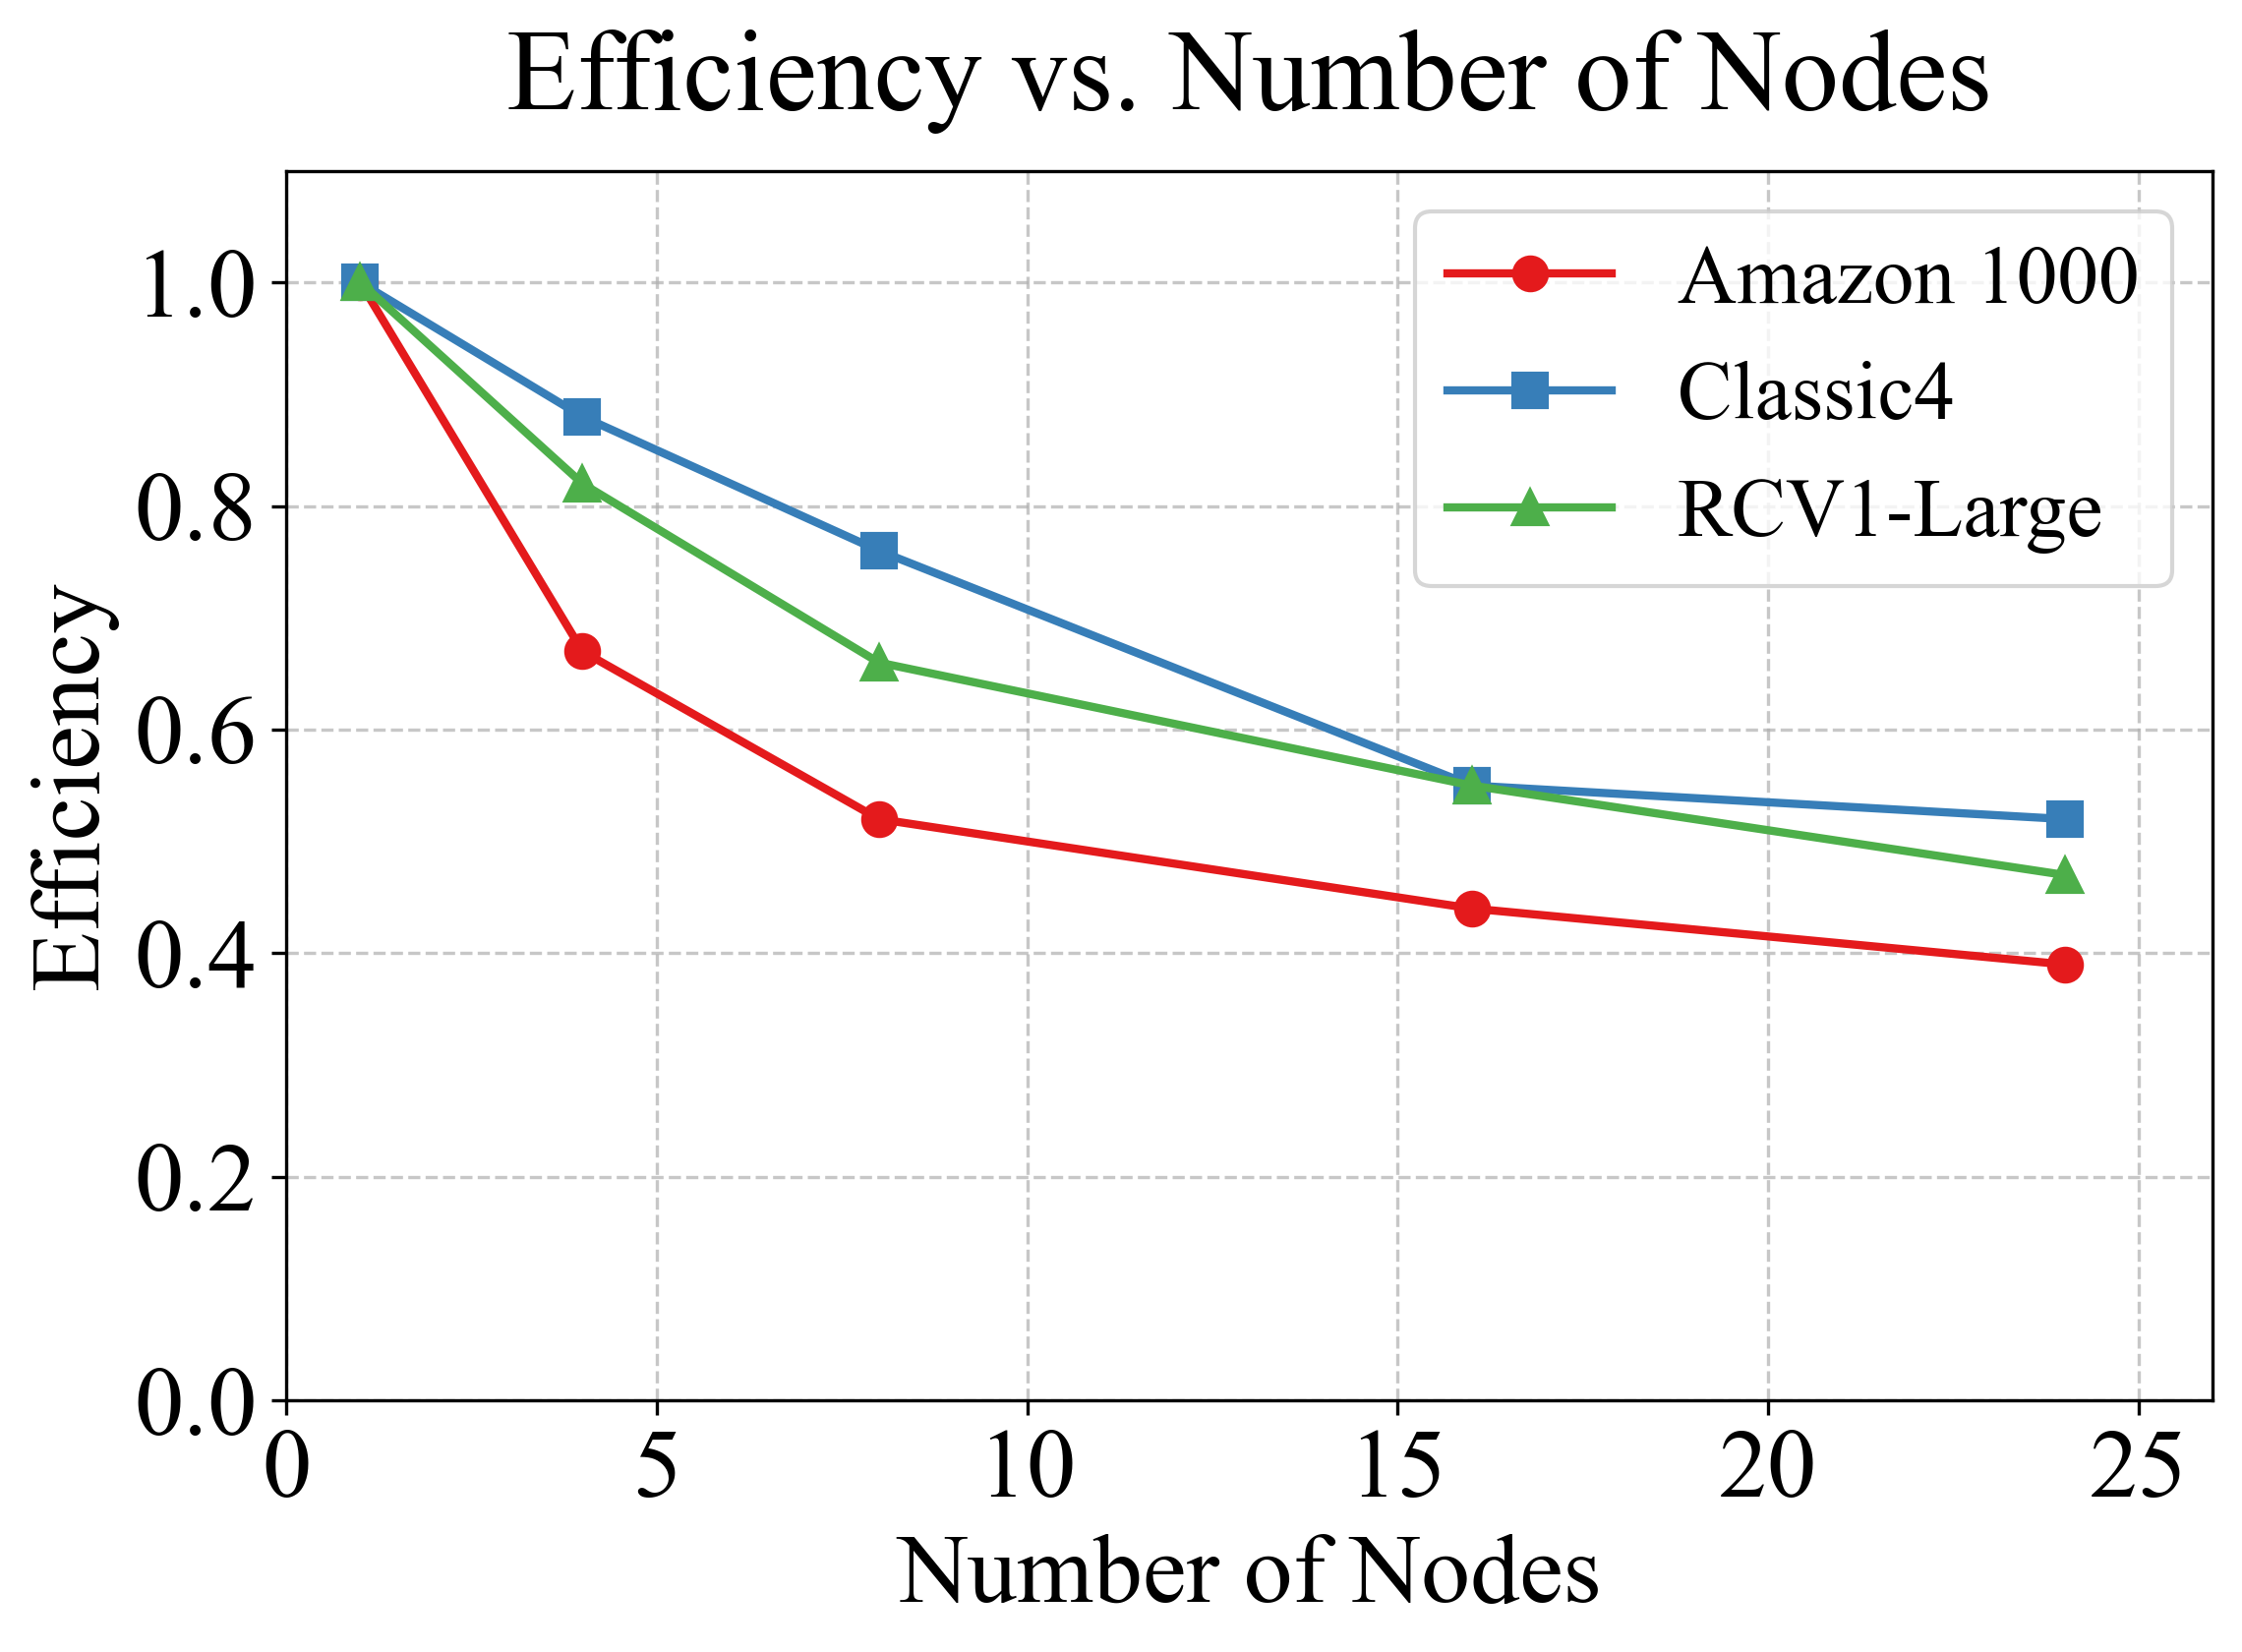
\includegraphics[width=0.8\linewidth]{efficiency.png}
    \caption{Enhanced efficiency of the proposed method in handling large-scale datasets.}
    \label{fig:efficiency}
\end{figure}

\Cref{fig:efficiency} presents the efficiency of our proposed co-clustering method across different datasets as the number of nodes increases. The datasets considered are Amazon 1000, CLASSIC4, and RCV1-Large. The x-axis represents the number of nodes, while the y-axis indicates the efficiency, normalized to the baseline (single node) efficiency of 1.


For Amazon 1000 Dataset, the efficiency starts at 1 for a single node and gradually decreases to 0.39 as the number of nodes increases to 24. The decrease in efficiency is relatively smooth, indicating that our method scales well but exhibits some overhead as more nodes are added. Despite the reduction in efficiency, the method maintains more than 39\% efficiency with 24 nodes, highlighting the robustness of the algorithm even at higher parallelization levels.

For CLASSIC4 Dataset, the efficiency for CLASSIC4 begins at 1 and decreases to 0.52 with 24 nodes. The drop in efficiency is more pronounced compared to the Amazon 1000 dataset, especially between 4 and 8 nodes, indicating a higher overhead for this dataset as the number of nodes increases. The method still retains more than half of the efficiency at 24 nodes, demonstrating good scalability.

For RCV1-Large Dataset, starting from an efficiency of 1, it decreases to 0.47 at 24 nodes. The decrease is relatively smooth, similar to the Amazon 1000 dataset, but with a slightly steeper decline. The method shows significant efficiency retention at higher node counts, indicating effective parallelization.

\subsection{Partitioning Parameter Analysis}
We analyzed the optimization of partition settings to determine the ideal balance between the number of partitions, the number of repetitions, and the computation time. The datasets were divided into varying numbers of partitions: 25, 36, 49, 81, 100, and 121. For each partition setting, the required number of repetitions and the corresponding computation time (in seconds) were recorded. The experiment aimed to identify the optimal partition setting that minimizes computation time while maintaining a feasible number of repetitions. The results, shown in \Cref{fig:optimisation}, highlight the optimal setting at 100 partitions, where computation time is minimized, and the number of repetitions remains stable.

\begin{figure}[htbp]
    \centering
    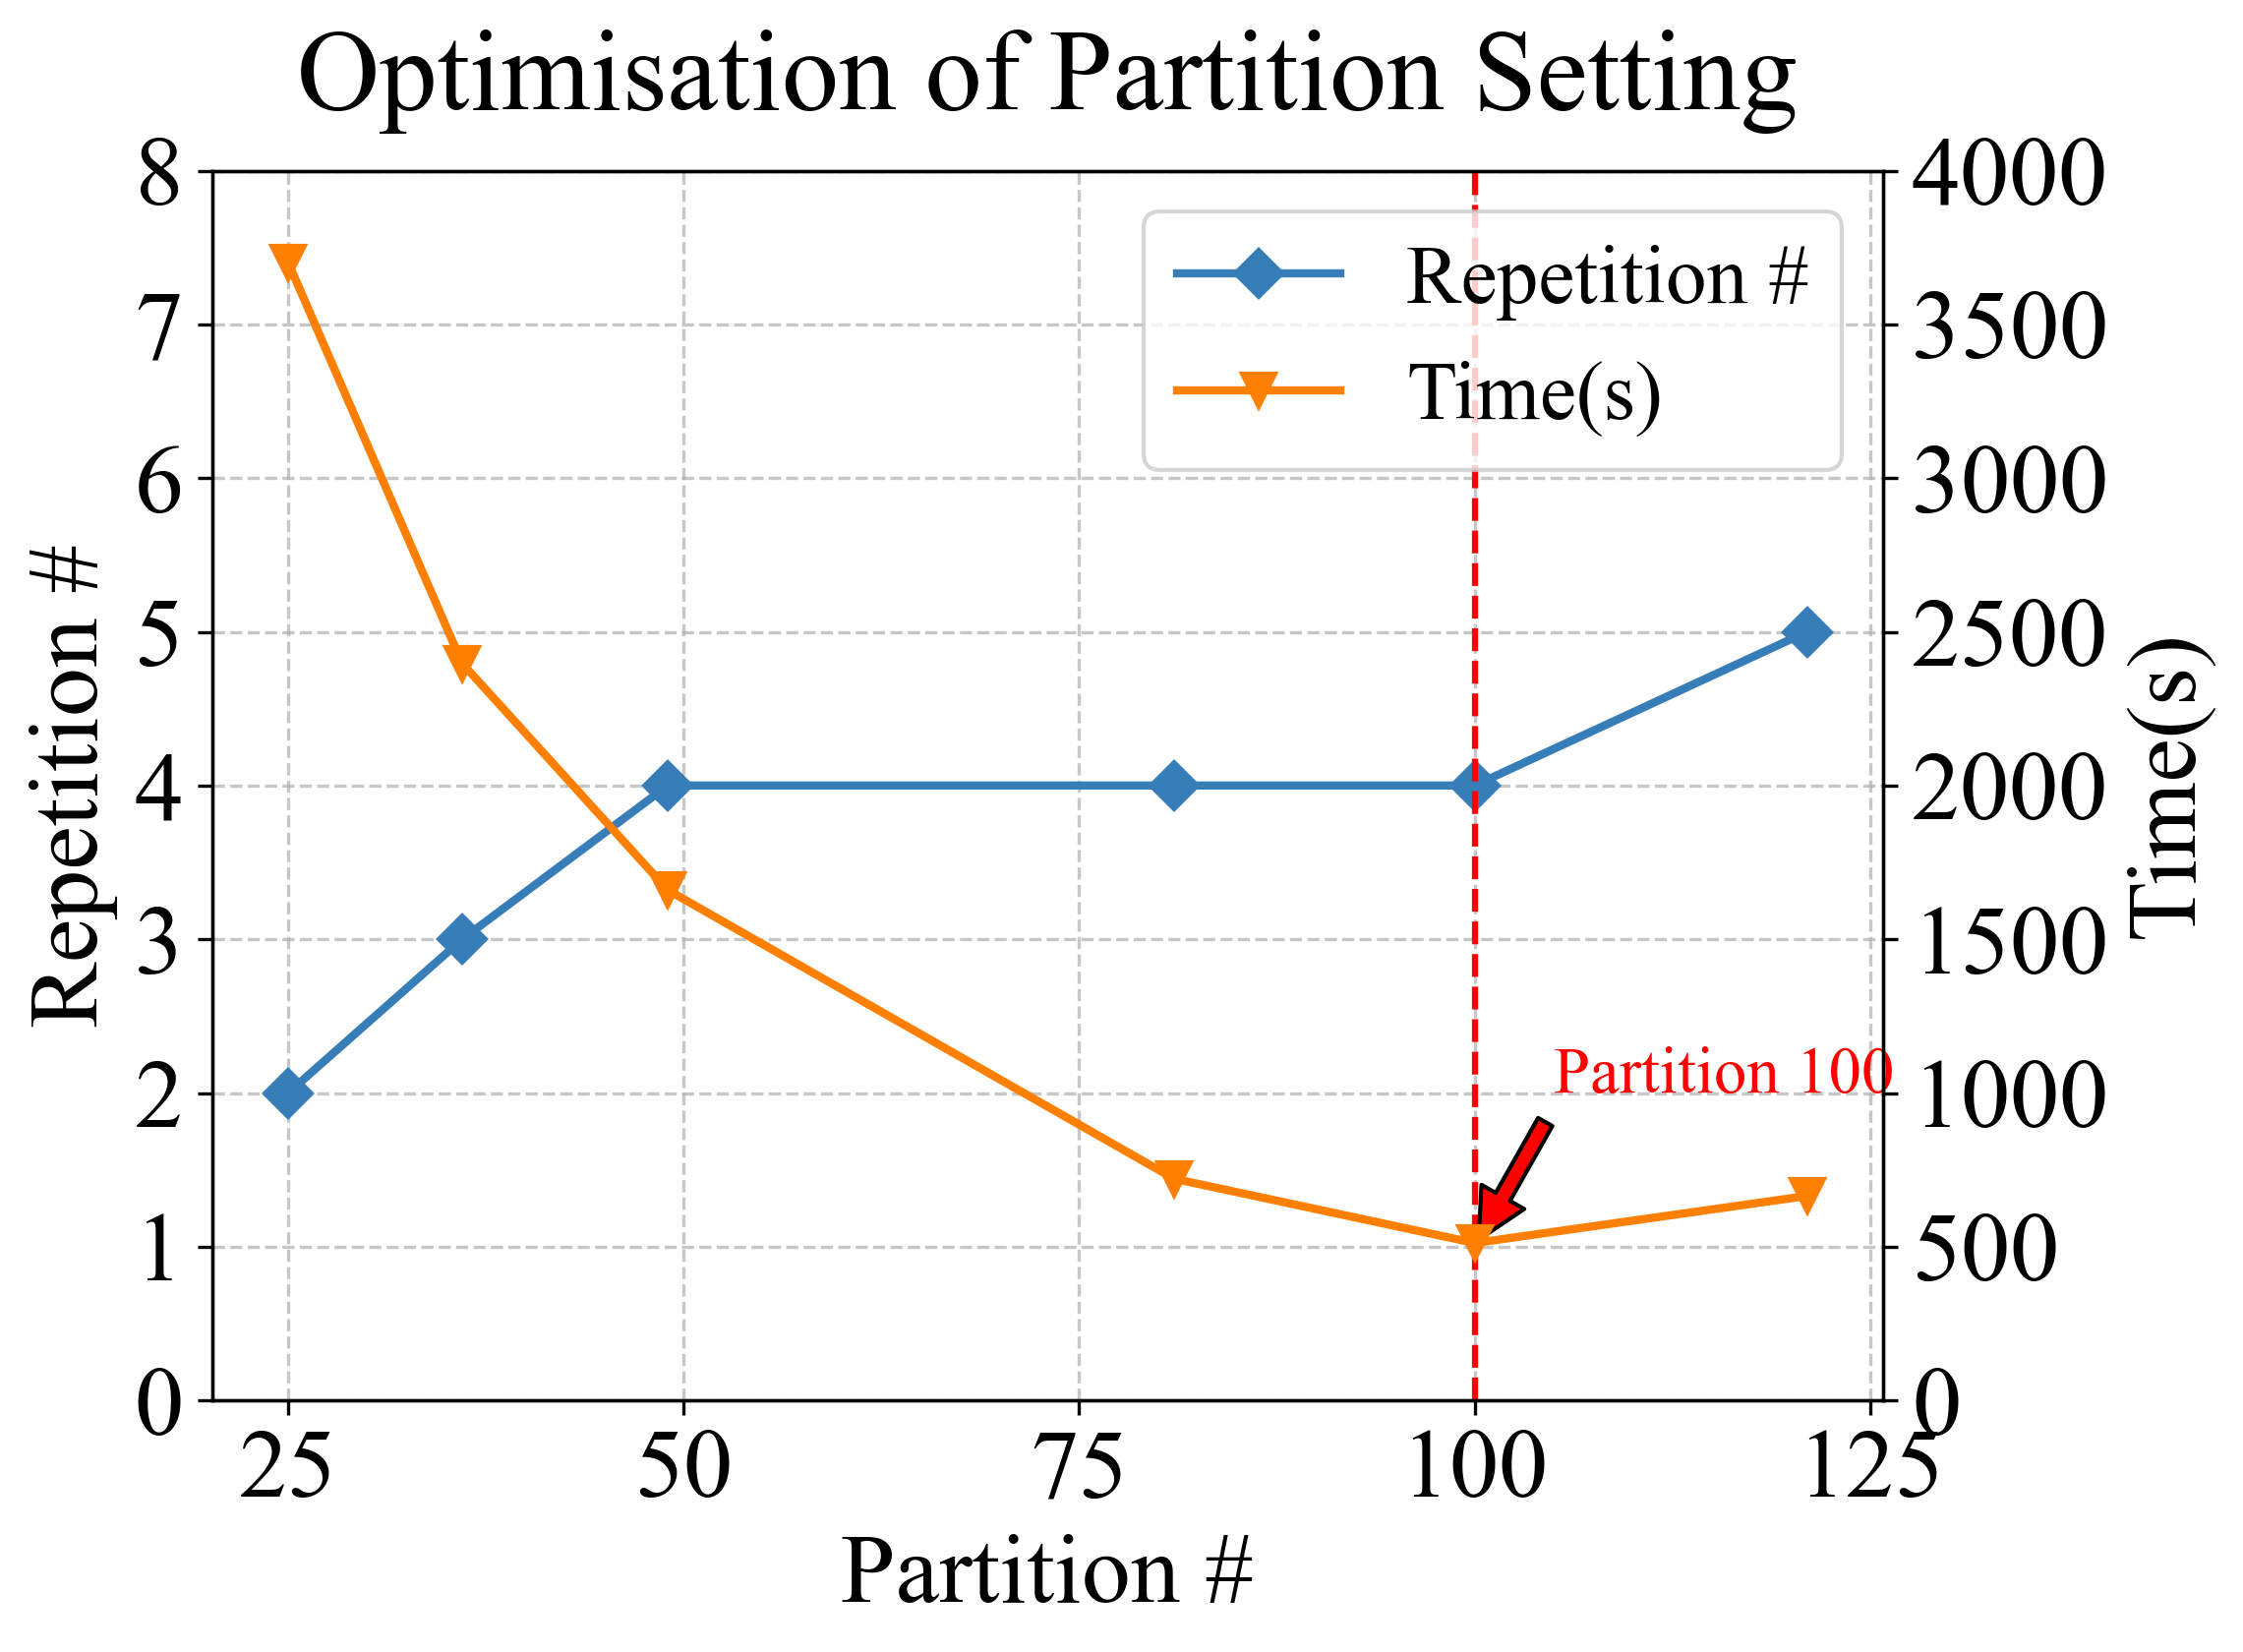
\includegraphics[width=0.8\linewidth]{optimisation.png}
    \caption{Optimization of the partitioning algorithm for computational efficiency.}
    \label{fig:optimisation}
\end{figure}

\subsubsection{Parameter Settings and Optimization}
\Cref{fig:optimisation} illustrates the relationship between the number of partitions, the number of repetitions, and the computation time (in seconds). The x-axis represents the number of partitions, while the primary y-axis indicates the number of repetitions, and the secondary y-axis shows the computation time in seconds.

The blue line represents the number of repetitions needed for different partition counts. As the number of partitions increases from 25 to 121, the number of repetitions initially rises, peaking at 4 for partitions 49, 81, and 100 before slightly increasing to 5 at 121 partitions. This trend suggests that more partitions generally require a higher number of repetitions to achieve optimal co-clustering, but there is a point of diminishing returns.

The orange line shows the computation time corresponding to different partition counts. There is a noticeable decrease in computation time as the number of partitions increases from 25 to 100, with the time dropping from 3,701 seconds to 512 seconds. However, the computation time slightly increases to 665 seconds at 121 partitions. This indicates that while increasing the number of partitions initially improves computational efficiency, beyond a certain point, the overhead of managing more partitions outweighs the benefits.

\subsubsection{Performance Impact Analysis}
The red dashed line at 100 partitions highlights the theoretical optimal setting, where the computation time is minimized. At this setting, the number of repetitions required is stable at 4, and the computation time is at its lowest. This confirms that our theoretical analysis aligns with empirical results, validating the effectiveness of our partitioning strategy.

The results indicate that there is an optimal balance between the number of partitions and the number of repetitions required. Too few partitions result in higher computation times due to the increased complexity within each partition, while too many partitions lead to increased overhead from managing numerous small partitions.

The significant reduction in computation time as the number of partitions increases up to 100 demonstrates the scalability of our method. This efficiency gain is crucial for processing large-scale datasets, where computational resources and time are often limiting factors. The slight increase in computation time beyond 100 partitions suggests that there is an optimal range for partition counts that maximizes efficiency without incurring excessive overhead.

The practical implication of these findings is that our proposed method can be effectively tuned for various datasets by adjusting the number of partitions. The theoretical optimal setting at 100 partitions provides a benchmark for achieving the best performance, but the method's flexibility allows for adjustments based on specific dataset characteristics and computational constraints.

These experiments validated that our Matrix Partitioned and Hierarchical Co-Cluster Merging is an efficient and accurate approach to analyzing large data matrices. The method's innovative partitioning strategy and ensemble clustering technique offer a new direction for scalable and precise co-clustering in data analysis.


\section{Related Work}
\label{sec:related_work}
\subsection{Classical Co-clustering Methods}
The concept of \emph{biclustering}, a special case of co-clustering for two-dimensional data, where both the rows and columns of data are clustered simultaneously, was first introduced by Hartigan~\cite{hartigan1972DirectClusteringData} to analyze gene expression data. This pioneering approach recognized the importance of simultaneously considering multiple dimensions of data to uncover more nuanced patterns.

Spectral Co-clustering with Singular Value Decomposition (SVD), introduced by Dhillon \textit{et al.}~\cite{dhillon2001CoclusteringDocumentsWords}, became widely adopted due to its straightforward implementation and effectiveness. This method leverages the mathematical properties of SVD to identify clusters by analyzing the principal components of the data matrix. Spectral co-clustering has since become a foundational technique, inspiring two main branches in co-clustering research: graph-based and matrix factorization-based approaches.

The most widely used graph-based co-clustering method is the Flexible Bipartite Graph Co-clustering (FBGPC)~\cite{chen2023FastFlexibleBipartitea}. FBGPC applies a flexible bipartite graph model directly to the original data, allowing for the simultaneous clustering of two distinct sets of objects, such as users and items in a recommendation system. This approach effectively captures the interactions between these sets, providing deeper insights into their relationships.

In contrast, Non-negative Matrix Tri-Factorization (NMTF)~\cite{long2005CoclusteringBlockValue} represents a leading matrix factorization-based method. NMTF decomposes the data matrix into multiple non-negative matrices, which correspond to the underlying factors of the data. By independently clustering both samples and features, NMTF reveals the latent structures within the data. This method has proven to be particularly useful in applications where the interpretability of factors is crucial, such as bioinformatics and social network analysis. Our method is orthogonal to NMTF, allowing for potential integration to enhance co-clustering efficiency.

Another innovative method, Deep Co-Clustering (DeepCC)~\cite{dongkuanxu2019DeepCoClustering}, combines the power of deep learning with traditional clustering techniques. DeepCC integrates deep autoencoders with Gaussian Mixture Models to improve the clustering of complex data. The autoencoders reduce the dimensionality of the data while preserving essential features, and the Gaussian Mixture Models identify clusters within this reduced space. Despite its advancements, DeepCC struggles with computational efficiency, particularly with diverse data types and iterative processes dependent on data sparsity. The deep learning components introduce additional layers of computation, which can be resource-intensive and time-consuming.

\subsection{Scalable Co-clustering Methods}
The emergence of big data has necessitated scalable co-clustering solutions, leading to developments in both distributed frameworks and parallel processing approaches. These advances aim to address the computational challenges inherent in processing massive datasets while maintaining clustering quality.

Co-ClusterD~\cite{cheng2015CoClusterDDistributedFramework} pioneered distributed co-clustering through Alternating Minimization Co-clustering (AMCC). While this approach enables parallel processing of data chunks, it faces fundamental challenges in maintaining convergence guarantees across distributed updates. The sequential dependencies in AMCC create processing bottlenecks, and communication overhead increases substantially with data dimensionality, limiting its effectiveness for very large datasets.

Parallel Non-negative Matrix Tri-Factorization (PNMTF)~\cite{chen2023ParallelNonNegativeMatrix} represents a significant advancement in parallel co-clustering by distributing matrix factorization across computing nodes. However, several critical limitations persist in PNMTF and similar approaches. The reliance on centralized control threads creates processing bottlenecks, while synchronization requirements introduce significant communication overhead. Moreover, the number of potential relationships to evaluate grows exponentially with data size, further challenging scalability.

Existing co-clustering algorithms~\cite{chen2023ParallelNonNegativeMatrix, cheng2015CoClusterDDistributedFramework} commonly rely on centralized processing for managing co-cluster statistics, creating bottlenecks that significantly limit their scalability. The dual-focus nature of co-clustering, which requires simultaneous optimization of row and column clusters, compounds these challenges by necessitating extensive relationship evaluations across the entire dataset.

Our work addresses these limitations through a novel divide-and-conquer strategy that fundamentally differs from existing approaches. By employing probabilistically-guided matrix partitioning, we preserve co-cluster integrity while enabling fully distributed processing with minimal synchronization requirements. Our hierarchical merging strategy maintains global structure while operating locally, effectively eliminating centralized bottlenecks while maintaining theoretical guarantees for co-cluster preservation. This approach provides a scalable solution that maintains clustering quality even for extremely large datasets.



\section{Conclusion}
\label{sec:conclusion}
We presented DiMergeCo, a scalable co-clustering method for large-scale datasets, leveraging a divide-and-conquer strategy to partition the input matrix into smaller submatrices for parallel processing, thereby significantly reducing computational overhead. Each submatrix is co-clustered independently using a probabilistic model-based optimal partitioning algorithm, ensuring the integrity of co-clusters, and the results are combined using a hierarchical co-cluster merging algorithm to enhance accuracy and reliability. Our implementation using MPI distributes the computational load across multiple nodes, improving scalability and making the approach practical for large-scale applications without requiring specialized performance from any single node. Experimental results demonstrate substantial improvements in computational efficiency and scalability, confirming the method's effectiveness for diverse and extensive datasets. This work addresses the challenges of co-clustering large-scale data by integrating efficient partitioning, parallel processing, and robust merging techniques, setting a new benchmark for scalable co-clustering and paving the way for future research in scalable data analysis technologies.

\printbibliography

\onecolumn
\newpage
\appendix
\section{Additional Theoretical Analysis}
\label{sec:appendix_theoretical_analysis}

This appendix provides a detailed account of the theoretical underpinnings of our proposed co-clustering framework. We present extended error bounds (\Cref{subsec:extended_error_bounds}), complexity analyses (\Cref{subsec:complexity_analysis}), and optimality conditions (\Cref{subsec:optimality_conditions}). We also include further technical lemmas and probability analyses (\Cref{subsec:probability_analysis}), along with detailed proofs (\Cref{subsec:detailed_proofs}).

\subsection{Extended Error Bounds}
\label{subsec:extended_error_bounds}

This section expands on the main text by giving precise statements and proofs of the error bounds that guarantee the quality of our divide-and-conquer approach.

\begin{theorem}[Global Error Bound]
    \label{thm:global_error_bound_appendix}
    Let \(\{\mathbf{B}_{(i,j)}\}\) be the submatrices after partitioning \(\mathbf{A}\), and let \(\hat{\mathbf{A}}\) be the reconstructed approximation from merging locally co-clustered results. If each block approximation error is bounded by \(\epsilon_{(i,j)}\), then
    \begin{equation}
        \|\mathbf{A} - \hat{\mathbf{A}}\|_F \;\le\; \sum_{i,j}\epsilon_{(i,j)}.
    \end{equation}
\end{theorem}

\begin{corollary}[Probabilistic Guarantee]
    \label{cor:prob_guarantee}
    If submatrices and the number of sampling/partitioning attempts \(T_p\) are chosen via the probabilistic model in Section~\ref{sec:proposed_model}, for any prescribed \(\delta\),
    \begin{equation}
        P\bigl(\|\mathbf{A} - \hat{\mathbf{A}}\|_F \;\le\; \delta\bigr) \;\ge\; 1 - \alpha,
    \end{equation}
    where \(\alpha\) can be made arbitrarily small by increasing \(T_p\) or refining the partition.
\end{corollary}

\begin{theorem}[Co-clustering Recovery Error]
    \label{thm:recovery_error_appendix}
    For each submatrix, if the local solution is \(\epsilon_{(i,j)}\)-optimal and the approximation error of that block is \(\delta_{(i,j)}\), then
    \begin{equation}
        \|\mathbf{F}' - \mathbf{F}^*\|_F \;\le\; \sum_{i,j}\epsilon_{(i,j)} \;+\; g\bigl(\{\delta_{(i,j)}\}\bigr),
    \end{equation}
    where \(\mathbf{F}^*\) is the global optimal solution and \(g\) captures how local approximation errors propagate globally.
\end{theorem}

The above results imply that if each subproblem is well-approximated and locally optimized, the merged global solution remains close to a global optimum.

\subsection{Complexity Analysis}
\label{subsec:complexity_analysis}

We now analyze the computational complexity and communication overhead of our framework.

\begin{lemma}[Computational Complexity]
    \label{lem:computational_complexity}
    Assume the original matrix is \(m \times n\), partitioned into \(p \times q\) blocks, each of size at most \(\phi_{\max} \times \psi_{\max}\). Running a local co-clustering algorithm of complexity \(O\bigl(f(\phi_{\max}, \psi_{\max})\bigr)\) on each block yields a total time complexity of
    \begin{equation}
        O\Bigl(\max_{(i,j)} f(\phi_i,\psi_j)\Bigr),
    \end{equation}
    assuming a balanced partition among processing nodes.
\end{lemma}

\begin{theorem}[Communication Complexity]
    \label{thm:communication_overhead}
    The communication overhead is bounded by \(O(K \log K)\), where \(K\) is the number of local co-clusters. This arises because only cluster assignments and summary statistics are exchanged during merging, rather than broadcasting large-scale intermediate factorizations.
\end{theorem}

The above results show that each node handles only a fraction of the data, thus drastically reducing both the per-node time and memory requirements.

\subsection{Optimality Conditions}
\label{subsec:optimality_conditions}

Although global optimality cannot be guaranteed for this non-convex co-clustering problem, the following conditions improve solution quality and increase the likelihood of approaching near-optimal solutions.

\begin{lemma}[Partition Refinement]
    \label{lem:partition_refinement}
    Refining the partition (i.e., increasing \(p\) and \(q\) so that submatrices become smaller) improves the local approximation by reducing the maximum block size \(\phi_{\max}\times\psi_{\max}\). If each block error is bounded by \(\delta_{(i,j)}\), then
    \begin{equation}
        \epsilon_{\text{local}} \;\le\; C \,\max_{i,j}\{\phi_i\psi_j\},
    \end{equation}
    where \(C\) is a constant depending on data distributions.
\end{lemma}

\begin{theorem}[Sampling Convergence]
    \label{thm:sampling_convergence_appendix}
    Increasing the number of random partitions \(T_p\) exponentially decreases the probability of missing a co-cluster. Specifically,
    \begin{equation}
        P(\text{miss any co-cluster} ) \;\le\; K\,\exp(-\gamma T_p),
    \end{equation}
    where \(K\) is the number of significant co-clusters and \(\gamma>0\) depends on partition parameters.
\end{theorem}

\begin{proposition}[Near-Optimality]
    \label{prop:near_optimality}
    The framework can be made arbitrarily close to a global optimum by increasing the partition granularity (making submatrices smaller), repeating the partitioning process more often (\(T_p\)), and using stronger local algorithms. Concretely, there exist \(\phi_i, \psi_j, T_p\) such that
    \begin{equation}
        \|\mathbf{F}' - \mathbf{F}^*\|_F \;\; \text{can be made arbitrarily small.}
    \end{equation}
\end{proposition}

\subsection{Probability Analysis and Additional Lemmas}
\label{subsec:probability_analysis}

The probability analysis clarifies how large co-clusters remain intact within at least one submatrix. Below, we restate crucial lemmas and assumptions used in our proofs.

\noindent\textbf{Notations.}
We assume \(\mathbf{A}\in \mathbb{R}^{M\times N}\) is partitioned into \(m\times n\) blocks of size \(\phi_i\times\psi_j\), forming block set \(\{\mathbf{B}_{(i,j)}\}\). Each co-cluster \(\mathbf{C}_k\) spans rows \(\{I_k\}\) and columns \(\{J_k\}\). Thresholds \(T_m\) and \(T_n\) denote minimum row and column sizes of interest, respectively.

\begin{lemma}[Joint Probability of Co-Cluster Size]
    \label{lemma:joint_prob_size}
    For a co-cluster \(\mathbf{C}_k\) in block \(\mathbf{B}_{(i,j)}\), the probability that \(\mathbf{C}_k\) is smaller than \(T_m\) in rows and \(T_n\) in columns within \(\mathbf{B}_{(i,j)}\) is bounded by
    \begin{equation}
        P\bigl(M_{(i,j)}^{(k)} < T_m,\; N_{(i,j)}^{(k)} < T_n \bigr)\;\;\le\;\; \exp\bigl\lbrack -2(\phi_i\,m\,(s^{(k)})^2\;+\;\psi_j\,n\,(t^{(k)})^2)\bigr\rbrack ,
    \end{equation}
    where \(s^{(k)}\) and \(t^{(k)}\) denote normalized cluster dimensions.
\end{lemma}

\begin{assumption}[Gaussian Noise Model]
    \label{assump:gaussian_noise}
    A noise matrix \(\mathbf{N}\) with mean \(0\) and variance \(\sigma^2\) is added to the hidden co-cluster matrix \(\mathbf{A}\), forming the observed \(\mathbf{B}=\mathbf{A}+\mathbf{N}\). Each \(n_{ij}\sim \mathcal{N}(0,\sigma^2)\) i.i.d. If \(\max(\|\mathbf{B}\|_1,\|\mathbf{B}^T\|_1)/\sigma^2\geq \lambda\), certain matrix concentration inequalities apply.
\end{assumption}

\begin{definition}[Co-Cluster Score Function]
    \label{def:cc_score}
    For a submatrix \(\mathbf{A}_{I,J}\subseteq\mathbf{A}\), define
    \begin{equation}
        S_{row}(\mathbf{A}_{I,J}),\quad S_{col}(\mathbf{A}_{I,J}),\quad \text{and } S(\mathbf{A}_{I,J})
    \end{equation}
    exactly as in Definition 4 of the main text. These metrics measure homogeneity by row and column blocks, respectively.
\end{definition}

\begin{theorem}[Expected Co-Cluster Score]
    \label{thm:expected_cc_score}
    With noise \(\mathbf{N}\) as in \Cref{assump:gaussian_noise}, one can bound the expected row and column scores of submatrix \(\mathbf{B}_{I,J}\) and their variances. For instance,
    \begin{equation}
        \mathbb{E}\bigl\lbrack S_{row}(I,J)\bigr\rbrack \;\ge\; |I||J|\Bigl(1\;-\;\exp\bigl\lbrack -2/\bigl(\alpha\,\max(\|\mathbf{B}\|_1,\|\mathbf{B}^T\|_1)\bigr\rbrack \Bigr),
    \end{equation}
    and similar bounds hold for \(\text{Var}\lbrack S_{row}(I,J)\rbrack \) and \(S_{col}(I,J)\).
\end{theorem}

\begin{theorem}[Chernoff Bound on Score Fluctuations]
    \label{thm:chernoff_score}
    Using Chernoff-type arguments, the probability that the submatrix co-cluster score \(S(I,J)\) deviates from its expectation by more than \(\epsilon\) is exponentially small in \(\epsilon^2\) and proportional to \(|I|\cdot|J|\). Formally,
    \begin{equation}
        P\Bigl(|S(I,J)-\mathbb{E}\lbrack S(I,J)\rbrack | > \epsilon\Bigr) \;\le\; \exp\Bigl(-\frac{\epsilon^2}{2|I||J|\sigma^2 \exp(-2/(\alpha\,\lambda))}\Bigr).
    \end{equation}
\end{theorem}

\subsection{Detailed Proofs}
\label{subsec:detailed_proofs}

We now present selected technical proofs referenced in the main text and earlier sections of this appendix.

\subsubsection{Proof of Lemma \ref{lem:computational_complexity}}
\begin{proof}
    Assume an algorithm $\mathcal{L}$ for local co-clustering has worst-case complexity $O\bigl(f(\phi_{\max},\psi_{\max})\bigr)$, where $\phi_{\max}$ and $\psi_{\max}$ are maximum block dimensions. Since the matrix is partitioned into at most $p\times q$ blocks, each block is processed independently. Hence, the total computational cost is bounded by $p\times q \times O\bigl(f(\phi_{\max},\psi_{\max})\bigr)$ if done sequentially, or $O\bigl(\max f(\phi_i,\psi_j)\bigr)$ if done fully in parallel. Balancing the partition ensures a similar scale of submatrix for each node, yielding the stated complexity.
\end{proof}

\subsubsection{Proof of Theorem \ref{thm:communication_overhead}}
\begin{proof}
    Communication cost arises primarily from merging partial co-clusters. If $K$ is the total number of partial co-clusters across blocks, each merge step involves comparing pairs or updating metadata in a priority queue. The maximum number of merges is $K-1$. Each merge can be handled in $O(\log K)$ if using a balanced tree or heap structure. Hence, $O(K\log K)$ is the dominating cost. We do not transmit large factorization data or entire blocks, only summary statistics, which remains $O(1)$ or $O(\log K)$ per merge. Thus, the overall communication overhead is $O(K\log K)$.
\end{proof}

\subsubsection{Proof of Lemma \ref{lemma:joint_prob_size}}
\begin{proof}
    We define $\phi_i,\psi_j$ as the block dimensions. By modeling the row and column assignments as Bernoulli trials and applying standard Chernoff/Hoefding bounds, we get the probability that a co-cluster $\mathbf{C}_k$ remains wholly or partially in $\mathbf{B}_{(i,j)}$. The result follows by bounding the overlap probabilities and simplifying via the exponential expression in the lemma statement.
\end{proof}

\noindent \textbf{(Further proofs and additional lemmas can follow similarly.)}

\vspace{1em}
\noindent
\textbf{Summary of Appendix.} We have provided an extended theoretical account of our co-clustering framework, covering error bounds, complexity analyses, probability arguments, and detailed proofs. These results ensure that our method (1) preserves significant co-clusters with high probability, (2) scales favorably in both memory and computation, (3) converges to a stable local optimum, and (4) allows tuning of parameters to approach near-optimal solutions for large-scale data.

\begin{theorem}
    \label{thm:probability_co_cluster_detection_fixed}
    If the matrix $\mathbf{A}$ is partitioned into $m \times n$ blocks, each with fixed sizes $\phi_i \times \psi_j$, and the probability of failing to detect co-cluster $\mathbf{C}_k$ in any block is $P(\omega_k)$, then
    \begin{equation}
        P(\omega_k) \le \exp \left\{ -2 \left\lbrack \phi m \left(s^{(k)}\right)^2 + \psi n \left(t^{(k)}\right)^2 \right\rbrack \right\}
    \end{equation}
    Given $T_p$ independent random partitioning attempts, the probability of detecting the co-cluster $C_k$ at least once is
    \begin{equation}
        P \ge 1 - \exp \left\{ -2 T_p \lbrack \phi m (s^{(k)})^2 + \psi n (t^{(k)})^2\rbrack  \right\}
    \end{equation}
\end{theorem}

\begin{proof}
    Consider co-cluster $C_k$ with dimensions $M^{(k)} \times N^{(k)}$ falling into a block $B_{(i,j)}$ of size $\phi_i \times \psi_j$. The probability of co-cluster $C_k$ being fragmented (i.e., not entirely contained within any single block) in a single partitioning attempt is denoted by $P(\omega_k)$.

    The preservation probability for co-cluster $C_k$ in a specific block $B_{(i,j)}$ is determined by the likelihood that all rows and columns of $C_k$ are captured within that block. Using Chernoff-type bounds, we derive the upper bound for the failure probability as follows:
    \begin{equation}
        P(\omega_k) \le \exp \left\{ -2 \left\lbrack \phi m \left(s^{(k)}\right)^2 + \psi n \left(t^{(k)}\right)^2 \right\rbrack \right\}
    \end{equation}
    where:
    \begin{align*}
        s^{(k)} & = \frac{M^{(k)}}{M} - \frac{T_m - 1}{\phi_i}, \\
        t^{(k)} & = \frac{N^{(k)}}{N} - \frac{T_n - 1}{\psi_j}.
    \end{align*}

    Here, \(s^{(k)}\) and \(t^{(k)}\) represent the normalized minimum row and column sizes required for co-cluster \(C_k\) to be preserved within a block.

    Considering $T_p$ independent random partitioning attempts, the probability that co-cluster $C_k$ fails to be detected in all attempts is \( P(\omega_k)^{T_p} \). Consequently, the probability of successfully detecting co-cluster $C_k$ in at least one of the $T_p$ attempts is:
    \begin{equation}
        P \ge 1 - \exp \left\{ -2 T_p \left\lbrack \phi m \left(s^{(k)}\right)^2 + \psi n \left(t^{(k)}\right)^2 \right\rbrack \right\}
    \end{equation}

    This inequality ensures that by selecting appropriate values for \(m, n, \phi_i, \psi_j,\) and \(T_p\), the probability \(P\) of detecting co-cluster \(C_k\) meets or exceeds a desired threshold \(P_{\text{thresh}}\).
\end{proof}

\end{document}
